% !Mode:: "TeX:UTF-8"
%!TEX program = xelatex
\documentclass{cumcm}

\usepackage{url}
\usepackage[ruled]{algorithm2e}
\usepackage{float}
\usepackage{booktabs}
\usepackage{longtable}
\usepackage{array}
\usepackage{calc}
\usepackage{placeins}
\usepackage{needspace}

\renewcommand{\algorithmcfname}{算法}
\providecommand{\tightlist}{%
  \setlength{\itemsep}{0pt}\setlength{\parskip}{0pt}}
\newcommand{\real}[1]{#1}
\numberwithin{figure}{section}
\numberwithin{table}{section}
\renewcommand{\thefigure}{\arabic{section}-\arabic{figure}}
\renewcommand{\thetable}{\arabic{section}-\arabic{table}}
\raggedbottom

\title{生产企业质量控制与生产决策模型（初稿）}

\begin{document}
\maketitle

% 以下位置将在后续定稿中补入：
% \begin{abstract} ... \keywords{...} \end{abstract}
% \section{问题重述}
% \section{问题分析}
% \section{模型的假设}
% \section{符号说明}
% 先将章节计数置为4，使四个已完成问题依次编号为第5至第8章。
\setcounter{section}{4}

\section{问题一的模型建立与求解}

\subsection{求解目标与模型选择}

问题一要求企业根据抽样检测结果判断供应商提供的一批零配件是否应当接收。设该批零配件真实但未知的次品率为 \(p\)，供应商给出的标称次品率为

\[
p_0=0.1.
\]

企业从该批零配件中随机抽取 \(n\) 件，并记录样本中的次品数 \(X\)。当 \(X\) 较大时，样本结果倾向于说明真实次品率超过标称值，企业应考虑拒收；当 \(X\) 较小时，样本结果倾向于说明真实次品率低于标称边界，企业可以考虑接收。因此，题目中的两种情形分别对应右尾判定和左尾判定，需要建立两个方向相反、彼此独立的单边检验。

样本次品数是离散变量，且临界点附近的尾概率将直接决定检测方案能否满足信度要求。考虑到枚举计算规模较小，本文采用精确二项分布进行计算，避免正态近似在尾部产生误差。

题目只给出了标称次品率和信度要求，没有给出需要重点识别的超标次品率、最低检验功效及具体检测成本函数。因此，信度条件只能确定给定样本量下的判定临界值，不能唯一确定最小检测数量。本文先利用精确二项尾概率确定不同样本量下的临界值，再根据临界样本比例标准差的边际改善程度选择推荐检测数量。

\subsection{抽样检测的二项分布模型}

设第 \(i\) 件零配件的检测结果为随机变量 \(Y_i\)，规定

\[
Y_i=
\begin{cases}
1, & \text{第 }i\text{ 件零配件为次品},\\
0, & \text{第 }i\text{ 件零配件为合格品}.
\end{cases}
\]

若该批零配件的真实次品率为 \(p\)，则

\[
P(Y_i=1)=p,\qquad P(Y_i=0)=1-p.
\]

抽检 \(n\) 件后，样本次品总数为

\[
X=\sum_{i=1}^{n}Y_i.
\]

在随机抽样、各件零配件具有相同次品概率且质量状态近似独立的条件下，有

\[
\boxed{X\sim B(n,p)}. \tag{1}
\]

样本中恰好出现 \(k\) 件次品的概率为

\[
P(X=k)=\binom{n}{k}p^k(1-p)^{n-k},
\qquad k=0,1,\ldots,n. \tag{2}
\]

由此可利用二项分布的左右尾概率衡量某类抽样结果在标称次品率下出现的可能性。

\subsection{信度的概率含义}

本文将信度理解为对错误决策概率的控制。设允许的最大错误概率为显著性水平 \(\alpha\)，则信度为

\[
\gamma=1-\alpha. \tag{3}
\]

对于第一种情形，错误决策是指零配件的真实次品率并未超过标称值 \(p_0\)，但样本中偶然出现较多次品，使企业错误地拒收该批零配件。因此，若规定 \(X\ge x_r\) 时拒收，则 95\% 信度对应

\[
P_{p_0}(X\ge x_r)\le0.05. \tag{4}
\]

对于第二种情形，错误决策是指零配件的真实次品率处于或高于标称边界 \(p_0\)，但样本中偶然出现较少次品，使企业错误地接收该批零配件。因此，若规定 \(X\le x_a\) 时接收，则 90\% 信度对应

\[
P_{p_0}(X\le x_a)\le0.10. \tag{5}
\]

二项尾概率不是信度本身，而是原假设成立时触发错误决策的概率。将该概率控制在 \(\alpha\) 以内，即得到不低于 \(1-\alpha\) 的信度保证。这里的信度表示重复使用相同抽样规则时对长期误判比例的控制，并不表示``本次结论正确的概率''。

\subsection{单边抽样判定模型}

\subsubsection{95\% 信度下的拒收模型}

为判断真实次品率是否超过标称值，建立假设

\[
H_0:p\le p_0,\qquad H_1:p>p_0. \tag{6}
\]

样本中的次品数越多，越支持 \(H_1\)，因此将拒收区域设置在二项分布右尾。设样本量为 \(n\) 时的拒收临界次品数为 \(x_r\)，规定

\[
X\ge x_r
\]

时拒收该批零配件。相应右尾概率为

\[
P_p(X\ge x_r)
=
\sum_{k=x_r}^{n}
\binom{n}{k}p^k(1-p)^{n-k}. \tag{7}
\]

该概率随真实次品率 \(p\) 增大而增大。因此，在原假设 \(p\le p_0\) 内，最大错误拒收概率出现在边界 \(p=p_0\)：

\[
\sup_{p\le p_0}P_p(X\ge x_r)
=P_{p_0}(X\ge x_r). \tag{8}
\]

为满足 95\% 信度要求，应有

\[
P_{p_0}(X\ge x_r)\le0.05.
\]

在满足概率约束的条件下，为使拒收区域尽可能宽，取最小可行临界值：

\[
\boxed{
x_r(n)=
\min\left\{
x:P_{p_0}(X\ge x)\le0.05
\right\}.
} \tag{9}
\]

\subsubsection{90\% 信度下的接收模型}

为判断样本是否能够提供支持真实次品率低于标称边界的证据，建立假设

\[
H_0:p\ge p_0,\qquad H_1:p<p_0. \tag{10}
\]

样本中的次品数越少，越支持 \(H_1\)，因此将接收区域设置在二项分布左尾。设接收临界值为 \(x_a\)，规定

\[
X\le x_a
\]

时接收该批零配件。相应左尾概率为

\[
P_p(X\le x_a)
=
\sum_{k=0}^{x_a}
\binom{n}{k}p^k(1-p)^{n-k}. \tag{11}
\]

该概率随真实次品率 \(p\) 增大而减小。因此，在原假设 \(p\ge p_0\) 内，最大错误接收概率出现在边界 \(p=p_0\)：

\[
\sup_{p\ge p_0}P_p(X\le x_a)
=P_{p_0}(X\le x_a). \tag{12}
\]

为满足 90\% 信度要求，应有

\[
P_{p_0}(X\le x_a)\le0.10.
\]

在满足概率约束的条件下，为使接收区域尽可能宽，取最大可行临界值：

\[
\boxed{
x_a(n)=
\max\left\{
x:P_{p_0}(X\le x)\le0.10
\right\}.
} \tag{13}
\]

严格地说，该检验提供的是支持 \(p<p_0\) 的单边统计证据，并不能从逻辑上证明真实次品率必然不超过 \(p_0\)。

\subsection{检测数量确定的必要性}

式（9）和式（13）能够为给定样本量确定相应临界值，但不能自动给出唯一的检测数量。例如，若只抽检 \(n=2\) 件，并规定两件均为次品时拒收，则

\[
P_{0.1}(X\ge2)=0.1^2=0.01<0.05.
\]

该方案形式上满足 95\% 信度要求，但当真实次品率为 \(p=0.2\) 时，其拒收概率也只有

\[
P_{0.2}(X\ge2)=0.2^2=0.04,
\]

检验能力很弱。因此，首个满足尾概率约束的样本量不能直接作为推荐检测数量。

若要严格求解最小样本量，还需要给定重点识别的备择次品率 \(p_1\) 及最低检验功效 \(1-\beta\)。由于题目未提供这些信息，本文采用临界样本比例波动的边际改善程度作为辅助选样依据。

\subsection{标准差收敛判据}

对每个可行样本量，定义临界样本比例

\[
\hat p(n)=\frac{x(n)}{n}, \tag{14}
\]

并以

\[
\sigma(n)
=
\sqrt{
\frac{\hat p(n)[1-\hat p(n)]}{n}
} \tag{15}
\]

衡量临界样本比例的波动程度。式（15）使用临界比例 \(x(n)/n\)，用于比较判定临界比例随样本量增加时的波动尺度，并不等同于在 \(p=p_0\) 处计算的固定抽样标准误。

为衡量检测数量从 \(n-1\) 增加至 \(n\) 后标准差的相对改善，定义

\[
g(n)
=
\frac{\sigma(n-1)-\sigma(n)}
{\sigma(n-1)}. \tag{16}
\]

由于临界次品数只能取整数，标准差曲线存在局部锯齿。本文先采用五点移动中位数对有效标准差序列进行平滑，再设置

\[
\epsilon=0.01,\qquad W=10.
\]

若平滑后的标准差相对下降率连续 10 次满足

\[
0\le g(n)<0.01, \tag{17}
\]

则认为曲线已经进入稳定下降区域，继续增加样本量带来的单步相对改善不足 1\%。取首个满足上述条件的稳定区间起点作为推荐检测数量。

\subsection{模型求解方法}

设置

\[
p_0=0.1,\qquad
\alpha_r=0.05,\qquad
\alpha_a=0.10,
\]

\[
n=1,2,\ldots,1000,
\]

\[
\epsilon=0.01,\qquad W=10.
\]

模型采用枚举法求解：

\begin{enumerate}
\def\labelenumi{\arabic{enumi}.}
\tightlist
\item
  依次枚举候选样本量 \(n\)；
\item
  对每个 \(n\)，从小到大搜索满足式（9）的拒收临界值 \(x_r(n)\)；
\item
  从大到小搜索满足式（13）的接收临界值 \(x_a(n)\)；
\item
  计算临界比例、标准差及相对下降率；
\item
  对有效标准差序列进行五点移动中位数平滑；
\item
  搜索连续满足式（17）的首个稳定区间；
\item
  输出推荐检测数量、临界次品数和边界概率。
\end{enumerate}

二项尾概率通过正则化不完全贝塔函数计算：

\[
P(X\ge k)=I_p(k,n-k+1), \tag{18}
\]

\[
P(X\le k)=I_{1-p}(n-k,k+1). \tag{19}
\]

该方法避免了直接计算较大组合数可能引起的数值问题。

\subsection{求解结果}

利用 MATLAB 对 \(n=1,2,\ldots,1000\) 进行枚举，得到拒收模型和接收模型的临界比例标准差曲线。

拒收模型的标准差在小样本阶段下降较快，随后逐渐趋于平缓，如图 5-1 所示。经五点移动中位数平滑后，从 \(n=85\) 开始的连续 10 个点均满足

\[
0\le g(n)<\epsilon=0.01.
\]

在 \(n=85\) 至 \(n=94\) 的稳定区间内，平滑标准差的单步相对下降率约为 0.30\% 至 1.00\%。因此取首个稳定区间的起点

\[
n_r=85
\]

作为拒收模型的推荐检测数量。

\begin{figure}[htbp]
  \centering
  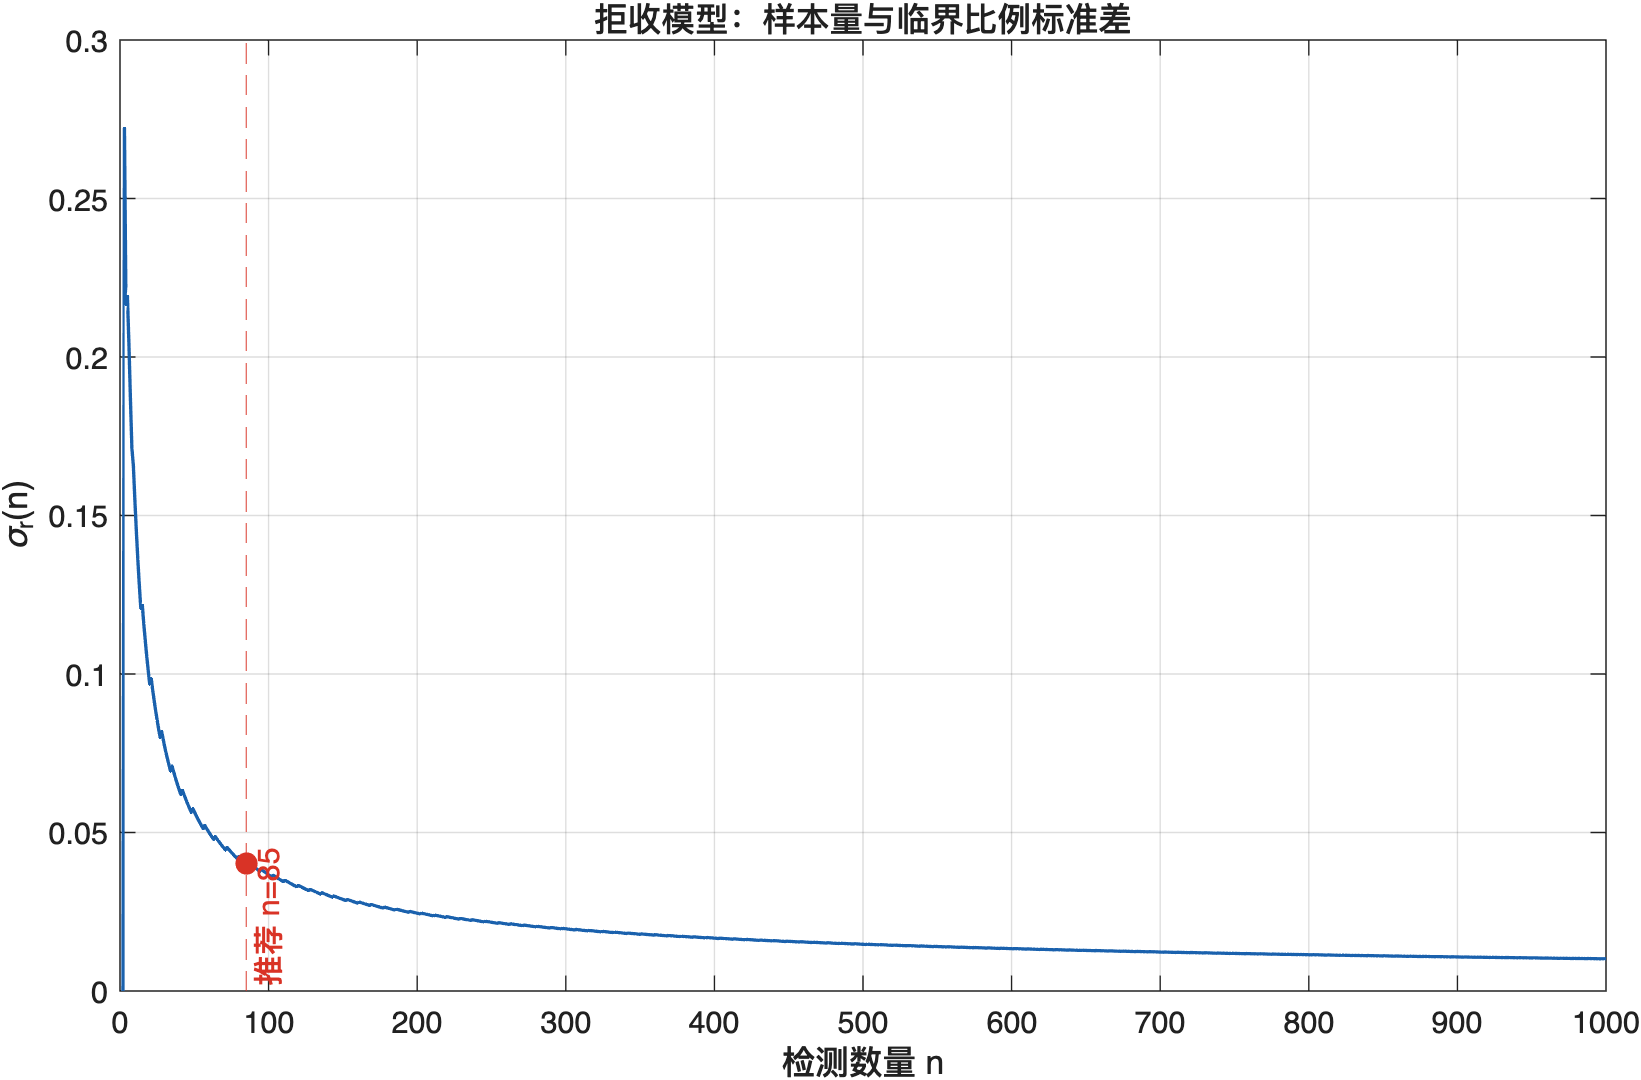
\includegraphics[width=0.86\linewidth]{../../第一问/results_problem1/reject_sigma_curve.png}
  \caption{拒收模型的检测数量与临界比例标准差曲线}
  \label{fig:p1-reject-sigma}
\end{figure}

接收模型受临界次品数整数变化影响，标准差曲线呈锯齿状下降，如图 5-2 所示。经平滑后，从 \(n=105\) 开始的连续 10 个点均满足相对下降率小于 1\% 的稳定条件。在 \(n=105\) 至 \(n=114\) 的稳定区间内，平滑标准差的单步相对下降率约为 0 至 0.91\%。因此取

\[
n_a=105
\]

作为接收模型的推荐检测数量。

\begin{figure}[htbp]
  \centering
  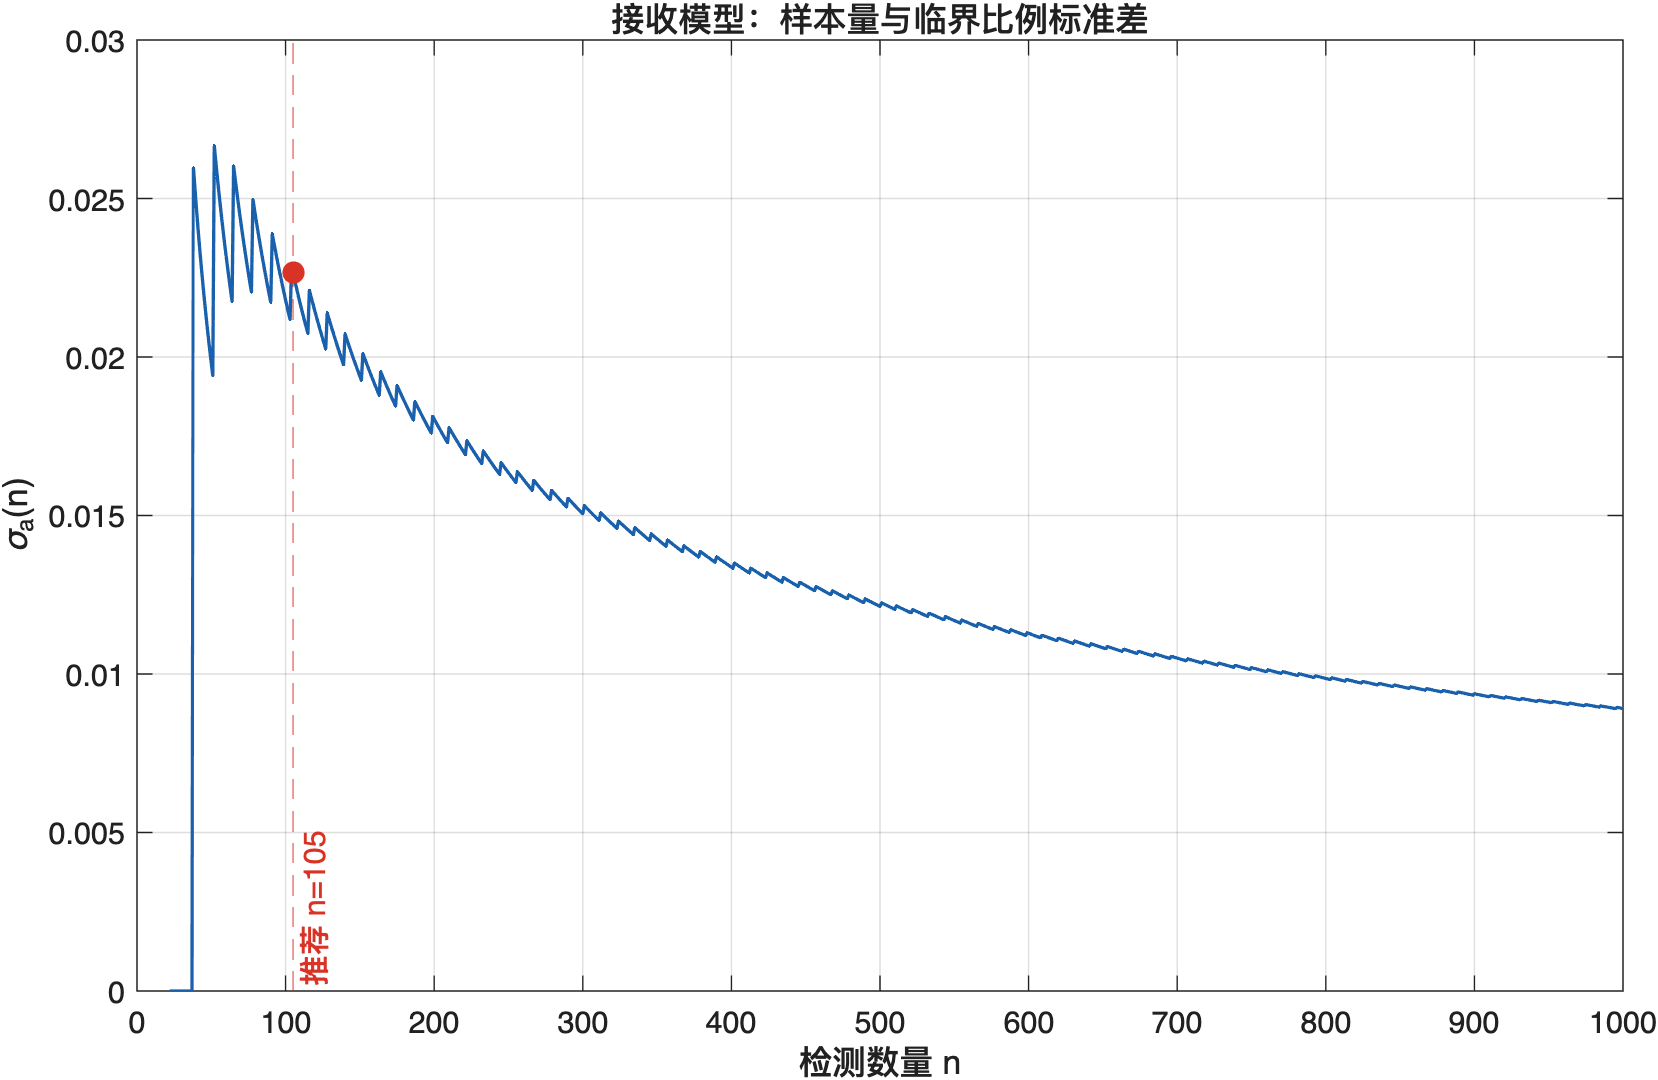
\includegraphics[width=0.86\linewidth]{../../第一问/results_problem1/accept_sigma_curve.png}
  \caption{接收模型的检测数量与临界比例标准差曲线}
  \label{fig:p1-accept-sigma}
\end{figure}

在上述样本量下，所得临界值及边界概率如下。

\clearpage
\begin{longtable}[]{@{}
  >{\raggedright\arraybackslash}p{(\linewidth - 8\tabcolsep) * \real{0.1667}}
  >{\raggedleft\arraybackslash}p{(\linewidth - 8\tabcolsep) * \real{0.2222}}
  >{\raggedleft\arraybackslash}p{(\linewidth - 8\tabcolsep) * \real{0.2222}}
  >{\raggedleft\arraybackslash}p{(\linewidth - 8\tabcolsep) * \real{0.2222}}
  >{\raggedright\arraybackslash}p{(\linewidth - 8\tabcolsep) * \real{0.1667}}@{}}
\caption{抽样检测方案及边界概率}\\
\toprule\noalign{}
\begin{minipage}[b]{\linewidth}\raggedright
判定情形
\end{minipage} & \begin{minipage}[b]{\linewidth}\raggedleft
检测数量 \(n\)
\end{minipage} & \begin{minipage}[b]{\linewidth}\raggedleft
临界次品数
\end{minipage} & \begin{minipage}[b]{\linewidth}\raggedleft
边界概率
\end{minipage} & \begin{minipage}[b]{\linewidth}\raggedright
判定规则
\end{minipage} \\
\midrule\noalign{}
\endfirsthead
\toprule\noalign{}
\begin{minipage}[b]{\linewidth}\raggedright
判定情形
\end{minipage} & \begin{minipage}[b]{\linewidth}\raggedleft
检测数量 \(n\)
\end{minipage} & \begin{minipage}[b]{\linewidth}\raggedleft
临界次品数
\end{minipage} & \begin{minipage}[b]{\linewidth}\raggedleft
边界概率
\end{minipage} & \begin{minipage}[b]{\linewidth}\raggedright
判定规则
\end{minipage} \\
\midrule\noalign{}
\endhead
\bottomrule\noalign{}
\endlastfoot
95\% 信度拒收 & 85 & \(x_r=14\) & \(P_{0.1}(X\ge14)=0.042310\) & \(X\ge14\) 时拒收 \\
90\% 信度接收 & 105 & \(x_a=6\) & \(P_{0.1}(X\le6)=0.089860\) & \(X\le6\) 时接收 \\
\end{longtable}

故问题一的抽样检测方案为

\[
\boxed{\text{抽检 85 件，若次品数不少于 14 件，则拒收该批零配件；}}
\]

\[
\boxed{\text{抽检 105 件，若次品数不多于 6 件，则接收该批零配件。}}
\]

\subsection{结果分析与模型检验}

\subsubsection{边界概率验证}

当真实次品率为标称值 \(p=0.1\) 时，85/14 方案触发拒收规则的概率为 4.231\%，小于规定的 5\%；105/6 方案触发接收规则的边界概率为 8.986\%，小于规定的 10\%。两套方案均满足相应的信度要求。

二项分布为离散分布，临界值只能取整数，实际尾概率通常无法恰好等于 0.05 或 0.10。本文所得概率略低于相应上限，说明精确检验在边界处具有一定保守性。

\subsubsection{操作特性分析}

不同真实次品率下，两套方案的判定概率如下。

\begin{longtable}[]{@{}rrr@{}}
\caption{不同真实次品率下两套方案的判定概率}\\
\toprule\noalign{}
真实次品率 \(p\) & 85/14 方案的拒收概率 & 105/6 方案的接收概率 \\
\midrule\noalign{}
\endfirsthead
\toprule\noalign{}
真实次品率 \(p\) & 85/14 方案的拒收概率 & 105/6 方案的接收概率 \\
\midrule\noalign{}
\endhead
\bottomrule\noalign{}
\endlastfoot
0.05 & 0.000080 & 0.727800 \\
0.08 & 0.007400 & 0.256012 \\
0.10 & 0.042310 & 0.089860 \\
0.12 & 0.136472 & 0.025400 \\
0.15 & 0.396925 & 0.002755 \\
0.20 & 0.828184 & 0.000034 \\
\end{longtable}

随着真实次品率提高，拒收概率持续增大，而接收概率迅速下降，变化方向符合模型预期。当 \(p=0.20\) 时，85/14 方案的拒收概率约为 82.82\%；当 \(p=0.15\) 时，拒收概率仅约为 39.69\%。因此，95\% 信度控制的是标称边界处的错误拒收概率，并不意味着所有 \(p>0.1\) 的批次都有 95\% 的概率被拒收。

同理，当 \(p=0.05\) 时，105/6 方案的接收概率约为 72.78\%，不能将 90\% 信度解释为所有低次品率批次均有 90\% 的接收概率。

\subsubsection{稳定性参数敏感性分析}

改变相对改善阈值 \(\epsilon\) 和连续窗口 \(W\) 后，部分结果如下。

\begin{longtable}[]{@{}
  >{\raggedleft\arraybackslash}p{(\linewidth - 6\tabcolsep) * \real{0.2500}}
  >{\raggedleft\arraybackslash}p{(\linewidth - 6\tabcolsep) * \real{0.2500}}
  >{\raggedleft\arraybackslash}p{(\linewidth - 6\tabcolsep) * \real{0.2500}}
  >{\raggedleft\arraybackslash}p{(\linewidth - 6\tabcolsep) * \real{0.2500}}@{}}
\caption{稳定性参数敏感性分析结果}\\
\toprule\noalign{}
\begin{minipage}[b]{\linewidth}\raggedleft
\(\epsilon\)
\end{minipage} & \begin{minipage}[b]{\linewidth}\raggedleft
\(W\)
\end{minipage} & \begin{minipage}[b]{\linewidth}\raggedleft
拒收方案 \((n_r,x_r)\)
\end{minipage} & \begin{minipage}[b]{\linewidth}\raggedleft
接收方案 \((n_a,x_a)\)
\end{minipage} \\
\midrule\noalign{}
\endfirsthead
\toprule\noalign{}
\begin{minipage}[b]{\linewidth}\raggedleft
\(\epsilon\)
\end{minipage} & \begin{minipage}[b]{\linewidth}\raggedleft
\(W\)
\end{minipage} & \begin{minipage}[b]{\linewidth}\raggedleft
拒收方案 \((n_r,x_r)\)
\end{minipage} & \begin{minipage}[b]{\linewidth}\raggedleft
接收方案 \((n_a,x_a)\)
\end{minipage} \\
\midrule\noalign{}
\endhead
\bottomrule\noalign{}
\endlastfoot
0.005 & 5 & \((167,24)\) & \((193,13)\) \\
0.005 & 10 & \((184,26)\) & \((200,14)\) \\
0.010 & 5 & \((62,11)\) & \((98,5)\) \\
0.010 & 10 & \((85,14)\) & \((105,6)\) \\
0.020 & 5 & \((41,8)\) & \((53,2)\) \\
0.020 & 10 & \((41,8)\) & \((53,2)\) \\
\end{longtable}

当 \(\epsilon\) 减小时，进入稳定区间的要求更严格，推荐检测数量明显增加。由此可见，给定样本量下的临界值由精确二项约束确定，而最终推荐样本量对稳定性参数存在一定敏感性。85 和 105 是默认参数下检测数量与临界比例波动之间的折中，不是由信度条件唯一确定的全局最优值。

\subsection{问题一结论}

本文将样本次品数建模为二项随机变量，并分别构造右尾拒收规则和左尾接收规则。模型中的信度通过限制原假设成立时触发错误决策的概率来实现：95\% 信度对应最大错误拒收概率不超过 0.05，90\% 信度对应最大边界错误接收概率不超过 0.10。

根据标准差曲线的收敛趋势及 \(\epsilon=0.01\)、\(W=10\) 的稳定判据，最终得到

\[
\boxed{\text{抽检 85 件，若次品数不少于 14 件，则拒收该批零配件；}}
\]

\[
\boxed{\text{抽检 105 件，若次品数不多于 6 件，则接收该批零配件。}}
\]

两套方案在标称边界处的尾概率分别为 0.042310 和 0.089860，均满足题目规定的信度要求。两种方案分别针对题目中的两种独立情形，不能直接拼接为同一次抽样中的三段判定规则。若企业能够进一步提供检测成本、重点识别的超标次品率和最低检验功效，可在此基础上建立带功效约束的最小样本量模型或序贯抽样模型。

\FloatBarrier

\section{问题二的建模与解决}

\subsection{问题分析}

\subsubsection{决策之间的耦合关系}

问题二要求企业针对六种生产情形，分别决定是否检测两种零配件、是否检测成品、是否拆解不合格品，以及是否检测并重新利用拆解所得零配件。上述决策并非彼此独立。零配件检测会改变进入装配环节的质量分布；成品检测决定不合格品在企业内部还是市场端被发现；拆解与回收又会改变下一轮装配所使用零配件的来源。因此，当前决策产生的结果会反馈到后续生产，构成``采购---检测---装配---交付---拆解---回收---再生产''的闭环过程。

若仅比较一次装配的收入与成本，便会遗漏不合格品引起的替换生产、重复装配以及回收件再利用等后续影响。为使不同策略具有统一的收益口径，本文将从企业开始组织生产，到最终向用户交付一件合格产品的全过程定义为一个生产周期。一个周期中允许发生多轮装配和拆解，但销售收入只计算一次，所有实际发生的采购、检测、装配、调换和拆解费用均计入周期成本。

\subsubsection{优化目标}

设完整决策策略为 \(S\)，采用该策略完成一个生产周期所得净收益为 \(R(S)\)。由于零配件质量和装配结果均具有随机性，同一策略在不同生产周期中的收益并不相同。因此，本问不以单次收益为评价依据，而以长期平均净收益作为决策标准，即

\[
S^*=\arg\max_{S\in\Omega}F(S),
\qquad
F(S)=E[R(S)],
\]

其中，\(\Omega\) 为全部有效策略构成的可行域。该目标同时考虑了质量风险和由质量问题引起的全部经济后果。

\subsubsection{模型思路}

针对闭环生产过程中存在的状态反馈，本文建立随机生产闭环模型，逐轮模拟零配件获取、装配、成品检测、市场退换以及拆解回收过程；采用蒙特卡洛方法估计每种策略的期望净收益；再以该估计值作为适应度，通过遗传算法搜索较优策略。

问题二仅包含两种零配件。经过无效决策修复后，实际不同的策略只有80种，因此可进一步遍历全部有效策略，并用更大的仿真样本进行统一复评。最终求解路线为

\[
\begin{aligned}
\text{策略编码}
&\longrightarrow\text{随机闭环仿真}
\longrightarrow\text{蒙特卡洛收益评价}\\
&\longrightarrow\text{遗传算法搜索}
\longrightarrow\text{全枚举复核}.
\end{aligned}
\]

其中，闭环模型负责描述生产机理，蒙特卡洛模拟负责计算策略收益，遗传算法和全枚举分别承担搜索与校验功能。

\subsection{模型准备}

\subsubsection{模型假设}

结合题设，对生产过程作如下处理：

\begin{enumerate}
\def\labelenumi{\arabic{enumi}.}
\tightlist
\item
  两种零配件的质量状态相互独立，检测结果完全准确；
\item
  任一零配件不合格时，装配成品必为不合格品；当两个零配件均合格时，成品仍以题给成品次品率发生装配失效；
\item
  拆解过程不改变零配件原有质量，拆解所得零配件没有额外残值，其价值仅体现为后续生产中节约的采购成本；
\item
  未经成品检测而流入市场的不合格品会被用户发现，企业承担题给调换损失并继续生产替换品；
\item
  不考虑产能、交货时间及库存持有成本，企业能够持续采购所需零配件。
\end{enumerate}

这些假设将随机来源限定为零配件质量和装配失效，使不同决策造成的成本差异能够在同一闭环内比较。

\subsubsection{主要符号}

\begin{longtable}[]{@{}clc@{}}
\caption{问题二模型的主要符号}\\
\toprule\noalign{}
符号 & 含义 & 单位 \\
\midrule\noalign{}
\endfirsthead
\toprule\noalign{}
符号 & 含义 & 单位 \\
\midrule\noalign{}
\endhead
\bottomrule\noalign{}
\endlastfoot
\(p_i\) & 零配件 \(i\) 的次品率 & --- \\
\(p_f\) & 合格零配件投入时的成品次品率 & --- \\
\(c_i\) & 零配件 \(i\) 的购买单价 & 元/件 \\
\(d_i\) & 零配件 \(i\) 的检测成本 & 元/件 \\
\(c_a\) & 单次装配成本 & 元/次 \\
\(d_f\) & 成品检测成本 & 元/件 \\
\(c_s\) & 不合格品拆解成本 & 元/件 \\
\(L\) & 不合格品进入市场造成的调换损失 & 元/件 \\
\(P\) & 一件产品的市场售价 & 元/件 \\
\(T\) & 完成一件合格交付所需的装配轮数 & 次 \\
\(R(S)\) & 策略 \(S\) 在一个生产周期内的净收益 & 元 \\
\end{longtable}

\subsubsection{策略编码与可行域压缩}

对零配件 \(i=1,2\)，定义新购件检测变量 \(x_i\)、回收件检测变量 \(r_i\) 和回收利用变量 \(u_i\)；定义成品检测变量 \(y\) 和不合格品拆解变量 \(z\)。所有变量均为0-1变量，取1表示执行相应操作，取0表示不执行。完整策略写为

\[
S=(x_1,x_2,y,z,r_1,r_2,u_1,u_2),
\]

其染色体表示为

\[
\boxed{x_1x_2\mid yz\mid r_1r_2\mid u_1u_2}.
\]

例如，编码 \texttt{10\textbar{}\allowbreak01\textbar{}\allowbreak01\textbar{}\allowbreak11} 表示：检测新购零配件1，不检测新购零配件2；不检测成品，拆解不合格品；回收件1不检测直接利用，回收件2检测后利用。

原始8位编码共有 \(2^8=256\) 种组合，但其中存在无效决策。若 \(z=0\)，生产过程中不会产生回收件，故应令 \(r_i=u_i=0\)；若 \(u_i=0\)，检测后仍废弃该回收件只会增加成本，故令 \(r_i=0\)。经过修复，不拆解时存在

\[
2^2\times2=8
\]

种有效策略；拆解时，每种回收件具有``废弃、直接利用、检测后利用''三种处理方式，故存在

\[
2^2\times2\times3^2=72
\]

种有效策略。因此，本问的可行策略总数为

\[
\boxed{|\Omega|=8+72=80}.
\]

\subsection{随机生产闭环模型的建立}

\subsubsection{零配件来源与检测}

设第 \(t\) 轮装配前，\(A_{i,t}=1\) 表示库存中存在可用于零配件 \(i\) 的回收件，\(Q_{i,t}\in\{0,1\}\) 表示该回收件的真实质量，其中1为合格。初始不存在回收库存，即

\[
A_{1,1}=A_{2,1}=0.
\]

每轮装配优先使用已有回收件；没有回收件时，再按策略采购新件。设投入第 \(t\) 轮装配的零配件质量为 \(G_{i,t}\)。

当 \(A_{i,t}=1\) 时，企业不再支付购买费用，并有

\[
G_{i,t}=Q_{i,t}.
\]

当 \(A_{i,t}=0\) 且 \(x_i=0\) 时，只购买一个新件并直接装配，故

\[
G_{i,t}\sim\operatorname{Bernoulli}(1-p_i),
\qquad
C_{i,t}^{\mathrm{source}}=c_i.
\]

当 \(A_{i,t}=0\) 且 \(x_i=1\) 时，对每次购入的零配件进行检测，若发现不合格则重新采购，直至获得合格件。设所需采购次数为 \(K_{i,t}\)，则

\[
K_{i,t}\sim\operatorname{Geometric}(1-p_i),
\qquad
P(K_{i,t}=k)=p_i^{k-1}(1-p_i),
\]

相应来源成本为

\[
C_{i,t}^{\mathrm{source}}=K_{i,t}(c_i+d_i),
\]

且此时 \(G_{i,t}=1\)。因此，零配件检测的经济作用是用重复采购与检测费用，换取进入装配环节的确定合格状态。

\subsubsection{成品质量生成}

每轮装配支付成本 \(c_a\)。令 \(B_t\) 表示两个投入零配件均合格时，装配过程是否成功，则

\[
B_t\sim\operatorname{Bernoulli}(1-p_f).
\]

根据题设质量关系，第 \(t\) 轮成品状态为

\[
\boxed{G_{f,t}=G_{1,t}G_{2,t}B_t}.
\]

该式将零配件缺陷和装配失效统一到同一成品质量变量中：只有两个零配件均合格且装配过程成功时，\(G_{f,t}=1\)。

\subsubsection{成品检测与市场反馈}

若 \(y=1\)，每轮支付成品检测费用 \(d_f\)。合格成品进入市场并结束生产周期，不合格品在企业内部被识别并进入处置环节。若 \(y=0\)，成品直接进入市场；当 \(G_{f,t}=0\) 时，企业支付调换损失 \(L\)，回收该不合格品并重新组织生产。因此，第 \(t\) 轮的成品检测费用与调换损失分别为

\[
C_t^{\mathrm{final}}=yd_f,
\]

\[
C_t^{\mathrm{return}}=(1-y)(1-G_{f,t})L.
\]

成品检测并不改变产品质量，它改变的是缺陷被发现的位置。当 \(d_f\) 较低而 \(L\) 较高时，将不合格品拦截在企业内部通常更有利。

\subsubsection{拆解回收与状态转移}

当 \(G_{f,t}=0\) 且 \(z=0\) 时，不合格品直接报废，下一轮不存在回收库存：

\[
A_{1,t+1}=A_{2,t+1}=0.
\]

当 \(G_{f,t}=0\) 且 \(z=1\) 时，企业支付拆解费用 \(c_s\)。拆出的零配件保持本轮装配前的质量 \(G_{i,t}\)，并根据 \((r_i,u_i)\) 进入下一轮：

\[
(A_{i,t+1},Q_{i,t+1})=
\begin{cases}
(0,0),&u_i=0,\\
(1,G_{i,t}),&u_i=1,\ r_i=0,\\
(G_{i,t},G_{i,t}),&u_i=1,\ r_i=1.
\end{cases}
\]

第三种情况下需额外支付检测费用 \(d_i\)，只有合格回收件能够进入下一轮库存。由此可见，拆解是否有利取决于回收件节约的未来采购费用能否覆盖拆解和回收检测成本；直接利用虽可节约检测费，但也可能把不合格件带入下一轮生产。

\subsubsection{周期成本与收益}

第 \(t\) 轮发生的总成本为

\[
\begin{aligned}
C_t={}&\sum_{i=1}^{2}C_{i,t}^{\mathrm{source}}+c_a+yd_f\\
&+(1-y)(1-G_{f,t})L\\
&+z(1-G_{f,t})c_s\\
&+z(1-G_{f,t})\sum_{i=1}^{2}u_ir_id_i.
\end{aligned}
\]

定义首次完成合格交付的轮次为

\[
T=\min\{t:G_{f,t}=1\}.
\]

同一订单的售价只计一次，一个生产周期的净收益为

\[
\boxed{R(S)=P-\sum_{t=1}^{T(S)}C_t(S)}.
\]

这一定义把零配件检测、成品检测、市场退换和拆解回收产生的即时成本与后续影响统一到同一目标函数中。

\subsection{模型求解}

\subsubsection{蒙特卡洛收益评价}

给定策略 \(S\) 后，独立模拟 \(N\) 个生产周期，得到收益样本 \(R_1(S),R_2(S),\ldots,R_N(S)\)。采用样本平均值估计期望净收益：

\[
\widehat F_N(S)=\frac{1}{N}\sum_{k=1}^{N}R_k(S).
\]

搜索阶段取 \(N=5000\)。收益均值的蒙特卡洛标准误差和95\%区间分别为

\[
SE(S)=\frac{s_R(S)}{\sqrt N},
\]

\[
CI_{95\%}(S)=\widehat F_N(S)\pm1.96SE(S),
\]

其中，\(s_R(S)\) 为收益样本标准差。该区间用于衡量有限仿真次数造成的数值波动，而非估计题给次品率的统计误差。

数值实现中，将单个生产周期的最大装配轮数设为100；超过上限仍未完成交付时施加10000元惩罚，以排除反复使用不合格回收件造成的坏状态循环。最终入选策略的闭环完成率均为1，因此该保护条件未改变最终策略。

\subsubsection{遗传算法搜索}

遗传算法以8位策略编码为个体，以 \(\widehat F_N(S)\) 为适应度。参数设置为：种群规模100，最大迭代次数200，交叉概率0.8，单个位变异概率0.03，锦标赛规模3，精英保留数2。求解过程为：

\begin{enumerate}
\def\labelenumi{\arabic{enumi}.}
\tightlist
\item
  随机生成初始策略种群，并按照6.2.3节规则修复无效决策；
\item
  对种群中的不同策略进行闭环仿真，计算平均净收益；
\item
  每次随机抽取3个个体，通过锦标赛选择父代；
\item
  采用均匀交叉重组不同生产环节的决策位；
\item
  对各决策位进行0-1变异，并再次修复无效编码；
\item
  保留当代收益最高的2个个体，直至达到200代；
\item
  每种情形独立运行10次，记录最优策略的重复命中情况。
\end{enumerate}

适应度可能为负，因此使用锦标赛选择可以避免轮盘赌选择中对负适应度进行平移处理。

\subsubsection{全策略复核}

遗传算法适用于后续多零件、多工序的高维决策，但问题二只有80种有效策略。为区分真实收益差异与蒙特卡洛抽样波动，本文对80种策略逐一进行100000次独立仿真，并以大样本复评均值最高的策略作为各情形的最终方案。该复核同时检验遗传算法是否搜索到高收益区域。

\subsection{模型结果与决策分析}

\subsubsection{最优策略}

各情形的最终策略及闭环运行指标见表6-2。

\begin{longtable}[]{@{}
  >{\raggedleft\arraybackslash}p{(\linewidth - 14\tabcolsep) * \real{0.1176}}
  >{\centering\arraybackslash}p{(\linewidth - 14\tabcolsep) * \real{0.1471}}
  >{\raggedleft\arraybackslash}p{(\linewidth - 14\tabcolsep) * \real{0.1176}}
  >{\centering\arraybackslash}p{(\linewidth - 14\tabcolsep) * \real{0.1471}}
  >{\raggedleft\arraybackslash}p{(\linewidth - 14\tabcolsep) * \real{0.1176}}
  >{\raggedleft\arraybackslash}p{(\linewidth - 14\tabcolsep) * \real{0.1176}}
  >{\raggedleft\arraybackslash}p{(\linewidth - 14\tabcolsep) * \real{0.1176}}
  >{\raggedleft\arraybackslash}p{(\linewidth - 14\tabcolsep) * \real{0.1176}}@{}}
\caption{六种生产情形的最优联合策略}\\
\toprule\noalign{}
\begin{minipage}[b]{\linewidth}\raggedleft
情形
\end{minipage} & \begin{minipage}[b]{\linewidth}\centering
最优染色体
\end{minipage} & \begin{minipage}[b]{\linewidth}\raggedleft
平均净收益/元
\end{minipage} & \begin{minipage}[b]{\linewidth}\centering
95\%蒙特卡洛区间/元
\end{minipage} & \begin{minipage}[b]{\linewidth}\raggedleft
平均装配次数
\end{minipage} & \begin{minipage}[b]{\linewidth}\raggedleft
平均退回次数
\end{minipage} & \begin{minipage}[b]{\linewidth}\raggedleft
平均拆解次数
\end{minipage} & \begin{minipage}[b]{\linewidth}\raggedleft
GA命中率
\end{minipage} \\
\midrule\noalign{}
\endfirsthead
\toprule\noalign{}
\begin{minipage}[b]{\linewidth}\raggedleft
情形
\end{minipage} & \begin{minipage}[b]{\linewidth}\centering
最优染色体
\end{minipage} & \begin{minipage}[b]{\linewidth}\raggedleft
平均净收益/元
\end{minipage} & \begin{minipage}[b]{\linewidth}\centering
95\%蒙特卡洛区间/元
\end{minipage} & \begin{minipage}[b]{\linewidth}\raggedleft
平均装配次数
\end{minipage} & \begin{minipage}[b]{\linewidth}\raggedleft
平均退回次数
\end{minipage} & \begin{minipage}[b]{\linewidth}\raggedleft
平均拆解次数
\end{minipage} & \begin{minipage}[b]{\linewidth}\raggedleft
GA命中率
\end{minipage} \\
\midrule\noalign{}
\endhead
\bottomrule\noalign{}
\endlastfoot
1 & \texttt{10\textbar{}\allowbreak01\textbar{}\allowbreak01\textbar{}\allowbreak11} & 18.8506 & {[}18.7559, 18.9453{]} & 1.22384 & 0.22384 & 0.22384 & 0.90 \\
2 & \texttt{11\textbar{}\allowbreak01\textbar{}\allowbreak00\textbar{}\allowbreak11} & 11.9228 & {[}11.8264, 12.0191{]} & 1.25093 & 0.25093 & 0.25093 & 1.00 \\
3 & \texttt{10\textbar{}\allowbreak11\textbar{}\allowbreak01\textbar{}\allowbreak11} & 16.5226 & {[}16.4364, 16.6088{]} & 1.22327 & 0 & 0.22327 & 0.50 \\
4 & \texttt{11\textbar{}\allowbreak11\textbar{}\allowbreak00\textbar{}\allowbreak11} & 14.7561 & {[}14.6742, 14.8380{]} & 1.25048 & 0 & 0.25048 & 0.70 \\
5 & \texttt{01\textbar{}\allowbreak01\textbar{}\allowbreak00\textbar{}\allowbreak01} & 16.3959 & {[}16.2900, 16.5018{]} & 1.23433 & 0.23433 & 0.23433 & 0.60 \\
6 & \texttt{00\textbar{}\allowbreak00\textbar{}\allowbreak00\textbar{}\allowbreak00} & 21.7821 & {[}21.6789, 21.8852{]} & 1.16363 & 0.16363 & 0 & 1.00 \\
\end{longtable}

六种最优策略的闭环完成率均为1。情形3和4选择检测成品，其平均市场退回次数为0；其余情形不检测成品，平均退回次数与平均额外装配次数相等，符合``不合格品进入市场后重新生产替换品''的闭环设定。

\subsubsection{零配件检测与回收决策}

情形1的策略为 \texttt{10\textbar{}\allowbreak01\textbar{}\allowbreak01\textbar{}\allowbreak11}。零配件1的购买价为4元，前端检测后发现不合格件所造成的废弃成本较低，因此选择检测；零配件2的购买价为18元，而调换损失仅为6元，对全部新购件进行检测并不经济。产品拆解后，零配件2无需重新支付18元购买费，只需支付3元检测费即可判断是否继续利用，故形成``新购件不检、回收件检测后利用''的差异化决策。

情形2和4均检测两种新购零配件。此时进入装配的零配件必然合格，成品失效只来自装配过程，拆出的零配件也保持合格，因此两个回收件均可不经检测直接利用。该结果表明：回收件是否需要再次检测，不仅取决于检测成本，还取决于其进入成品之前是否已经接受过质量筛选。

情形5的策略为 \texttt{01\textbar{}\allowbreak01\textbar{}\allowbreak00\textbar{}\allowbreak01}。零配件1检测费为8元，高于其4元购买价，检测与回收均不具有成本优势；零配件2购买价为18元而检测费仅为1元，适合在采购端检测，并在拆解后直接利用。此时两种零配件采用不同策略，说明统一的``全部检测''或``全部不检测''规则不能替代逐零配件决策。

\subsubsection{成品检测与拆解决策}

情形1和3的零配件参数相近，但调换损失分别为6元和30元。情形1不检测成品，而情形3选择检测成品，并将平均市场退回次数由约0.22次降至0。由此可见，成品检测的作用不是提高产品合格率，而是用确定的检测费用替代不合格品流入市场后的高额损失。

情形6的三类次品率均为5\%，而拆解成本达到40元。低质量风险使检测的预期收益较小，高拆解费用又使回收节约无法覆盖处置成本，因此最优策略为 \texttt{00\textbar{}\allowbreak00\textbar{}\allowbreak00\textbar{}\allowbreak00}，即不检测、不拆解。该情形给出了闭环回收模型的一个经济边界：回收在物理上可行，并不意味着在成本上必然合理。

\subsubsection{遗传算法收敛特征}

图6-1给出了六种情形下一次代表性运行的当代最优适应度。各曲线在前若干代完成主要提升，随后保持不下降，200代足以覆盖本问的搜索需要。

\begin{figure}[htbp]
  \centering
  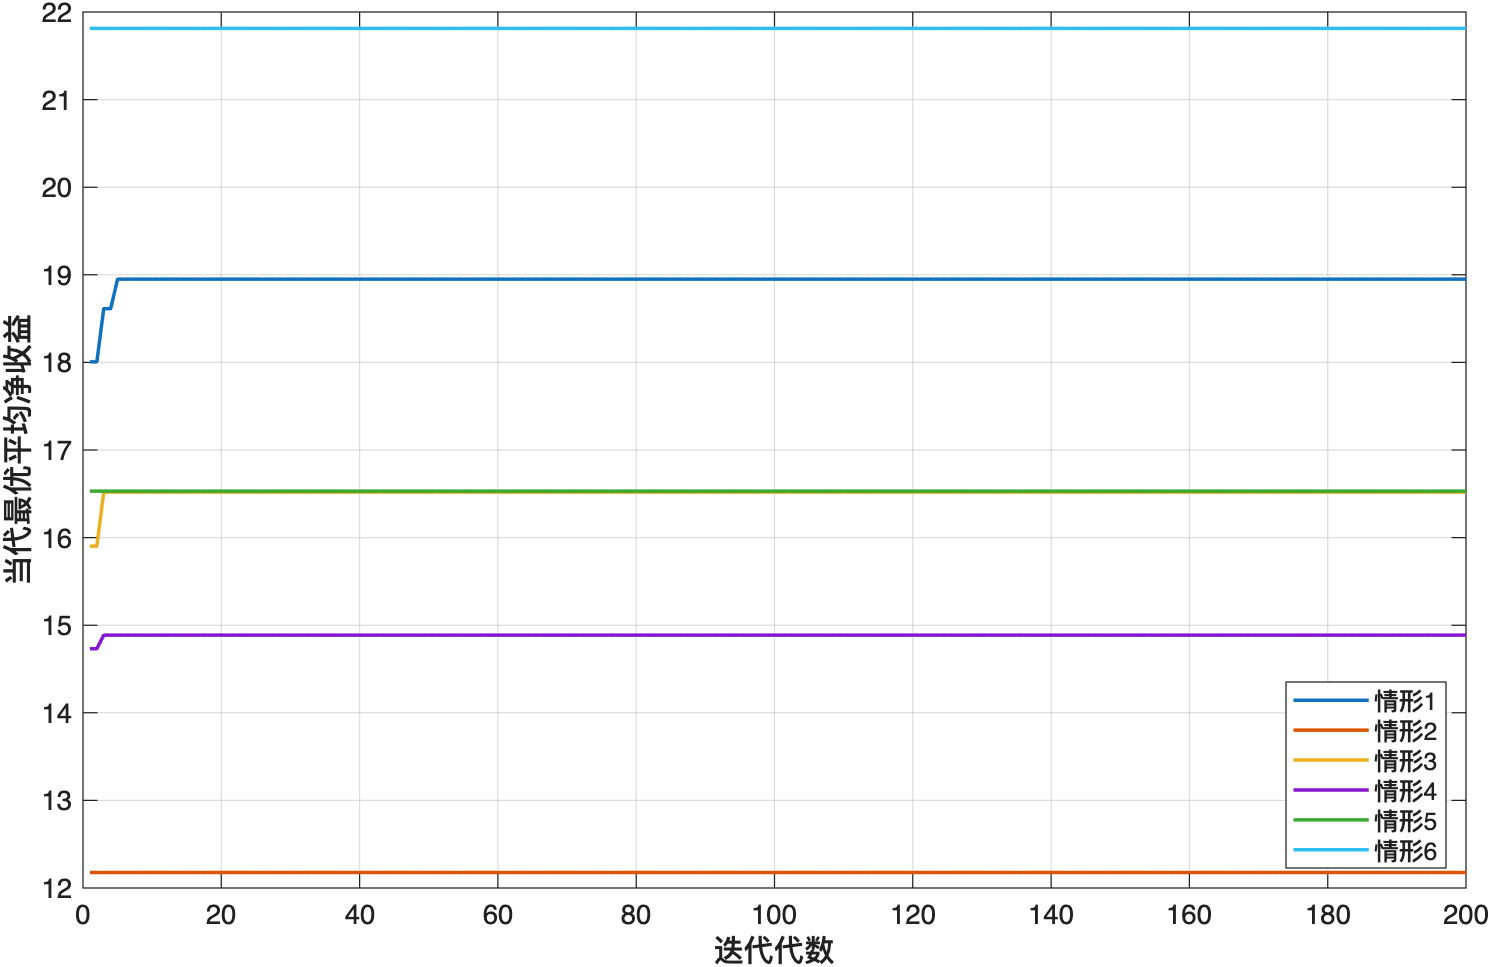
\includegraphics[width=0.86\linewidth]{../../第二问/results/ga_convergence.png}
  \caption{六种情形下遗传算法的最优适应度收敛曲线}
  \label{fig:p2-ga}
\end{figure}

曲线后期不下降是精英保留直接保留当代最优策略的结果。情形2和6从初始种群开始即处于稳定区间，而情形1、3和4在少数几代内完成策略改进。由于本问的有效策略空间较小，收敛速度本身不能证明所得方案为全局最优，最终结论仍以80种策略的大样本复评为准。

\subsection{模型检验}

\subsubsection{理论一致性检验}

当两种新购零配件均被检测时，进入装配环节的零配件均为合格件，成品每轮成功概率为 \(1-p_f\)。完成合格交付所需装配次数应服从几何分布，其理论均值为

\[
E[T]=\frac{1}{1-p_f}.
\]

情形2和4均有 \(p_f=0.2\)，故理论平均装配次数为1.25；仿真结果分别为1.25093和1.25048，相对偏差分别约为0.074\%和0.038\%。理论值与仿真值吻合，验证了零配件筛选、装配失效和闭环终止之间的状态关系。

\subsubsection{搜索稳定性检验}

10次独立遗传算法对六种情形最终策略的命中次数依次为9、10、5、7、6和10次。情形3和5的命中率分别为0.50和0.60，说明若仅采用5000次仿真计算适应度，收益相近的候选策略之间可能出现排序交换。对全部80种策略增加至100000次仿真后，可明显减小均值估计误差，因此表6-2采用复评结果而非单次GA输出。

\subsubsection{参数敏感性分析}

分别将六种情形中的全部次品率和调换损失上下扰动20\%，每次扰动后重新优化80种策略，共形成24个测试场景。其中20个场景保持原最优编码，策略保持率为

\[
\frac{20}{24}=83.33\%.
\]

情形1、2和4在四类扰动下均保持原策略。情形3在次品率下降20\%时取消新购件检测，但仍检测成品和回收件；情形5在次品率或调换损失上升20\%时转为检测成品；情形6在次品率上升20\%时开始检测零配件1，但仍不检测成品且不拆解。

敏感性结果说明，情形1、2和4的决策在给定扰动范围内较为稳定；情形3、5和6位于若干检测决策的切换边界附近。在问题四考虑次品率抽样误差时，应重点对后三种情形采用区间参数重新评价。

\subsection{本问结论}

本文以``完成一件合格产品交付''为统一生产周期，建立了覆盖采购、检测、装配、市场退换、拆解和回收利用的随机生产闭环模型，并通过蒙特卡洛模拟估计策略的长期平均净收益。遗传算法给出候选优良策略，再由80种有效策略的全枚举大样本复评确定最终方案。

六种情形的最优编码依次为 \texttt{10\textbar{}\allowbreak01\textbar{}\allowbreak01\textbar{}\allowbreak11}、\texttt{11\textbar{}\allowbreak01\textbar{}\allowbreak00\textbar{}\allowbreak11}、\texttt{10\textbar{}\allowbreak11\textbar{}\allowbreak01\textbar{}\allowbreak11}、\texttt{11\textbar{}\allowbreak11\textbar{}\allowbreak00\textbar{}\allowbreak11}、\texttt{01\textbar{}\allowbreak01\textbar{}\allowbreak00\textbar{}\allowbreak01} 和 \texttt{00\textbar{}\allowbreak00\textbar{}\allowbreak00\textbar{}\allowbreak00}，对应平均净收益分别为18.8506元、11.9228元、16.5226元、14.7561元、16.3959元和21.7821元。结果表明，调换损失升高会促使企业将质量控制前移至成品检测环节；购买价较高且检测费较低的零配件更适合检测和回收利用；拆解成本过高时，放弃回收反而能够获得更高收益。该闭环状态转移和收益评价框架可在问题三中继续扩展到多零配件和多道工序。

\FloatBarrier

\section{问题三的建模与解决}

\subsection{问题分析与模型扩展}

\subsubsection{两层装配结构}

问题三将问题二的单层装配扩展为两道工序：零配件1---3组成半成品1，零配件4---6组成半成品2，零配件7---8组成半成品3，三个半成品再装配为成品。相应装配拓扑为

\[
\mathcal G_1=\{1,2,3\},\qquad
\mathcal G_2=\{4,5,6\},\qquad
\mathcal G_3=\{7,8\},
\]

\[
\mathcal G_j\longrightarrow \text{半成品 }j,
\qquad
\{\text{半成品1,2,3}\}\longrightarrow\text{成品}.
\]

多一层装配后，缺陷可能由零配件、半成品装配或成品装配产生；不合格品的回收也形成两条路径：不合格半成品可拆为零配件，不合格成品可先拆为半成品，其中的不合格半成品还可继续拆为零配件。因此，企业不仅需要选择检测位置，还需决定质量信息如何随回收对象进入下一轮生产。

\subsubsection{与问题二的继承关系}

本文沿用问题二的收益口径，将``开始组织生产至最终完成一件合格交付''作为一个更新周期。同一订单只计算一次销售收入，周期内发生的重复采购、两层装配、检测、市场调换和拆解费用均计入成本。零配件、半成品与成品的质量状态具有随机性，故仍以策略的期望周期净收益为优化目标。

问题三新增半成品库存、半成品内部零配件质量以及两级拆解状态。若采用解析期望，需要枚举不同层次的已知与未知质量组合；若采用动态规划，状态数会随库存质量和循环轮次迅速增长。为保留完整生产机理并与问题二保持统一，本文将原随机生产闭环扩展为分层随机生产闭环，通过蒙特卡洛模拟评价策略，再用遗传算法搜索高收益方案。

\subsubsection{模型边界}

本文认为各零配件质量和各层装配失效事件相互独立，检测完全准确，拆解不改变组成对象的质量。正品零配件投入后，半成品仍按题给次品率发生装配失效；正品半成品投入后，成品亦按题给次品率发生装配失效。未经成品检测而进入市场的不合格品视为被用户发现并退回。不考虑产能、交货期和库存持有成本，回收件的价值体现为节约后续采购或装配费用。

\subsection{决策变量与策略编码}

\subsubsection{染色体构造}

完整策略编码为

\[
X(8)\mid H(3)\mid Y\mid D(3)\mid Z
\mid R(8)\mid U(8)\mid S(3)\mid V(3)
\]

其中，\(X,H,Y\) 分别表示新购零配件、半成品和成品检测；\(D,Z\) 表示半成品和成品拆解；\(R,U\) 表示回收零配件检测和利用；\(S,V\) 表示回收半成品检测和利用。染色体共含

\[
8+3+1+3+1+8+8+3+3=38
\]

个二进制位，未经修复的策略空间为

\[
2^{38}=274877906944.
\]

该规模无法沿用问题二的全枚举复核，需要采用启发式搜索。

\subsubsection{无效编码修复}

根据生产逻辑对染色体执行以下修复：若半成品 \(j\) 不拆解，则对应组内回收零配件的检测和利用位均归零；若某回收对象不利用，则其检测位归零；若成品不拆解，则回收半成品的检测和利用位均归零。

检测准确且拆解无损时，还存在两条支配规则。若 \(x_i=1\)，零配件 \(i\) 在进入装配前已经检测合格，拆解后的重复检测只增加成本，故令 \(r_i=0\)；若 \(h_j=1\)，半成品 \(j\) 已经检测合格，成品拆解后无需再次检测，故令 \(s_j=0\)。上述修复删除了行为相同或严格劣势的编码，不改变可实现的高收益策略。

\subsection{分层随机生产闭环模型}

\subsubsection{回收库存状态}

设 \(A_{i,t}^{(p)}=1\) 表示第 \(t\) 轮开始时存在回收零配件 \(i\)，\(Q_{i,t}^{(p)}\) 为其真实质量；\(A_{j,t}^{(s)}=1\) 表示存在回收半成品 \(j\)，\(Q_{j,t}^{(s)}\) 为其真实质量。由于回收半成品后续可能继续拆解，模型同时保留其内部各零配件的真实质量。初始没有回收库存：

\[
A_{i,1}^{(p)}=0,\qquad A_{j,1}^{(s)}=0.
\]

每轮生产优先使用回收对象；没有相应库存时，再采购零配件或重新装配半成品。

\subsubsection{零配件获取}

当存在回收零配件时，企业不再支付购买费用，投入质量由库存状态决定。若没有回收件且 \(x_i=0\)，只购买一个新件并直接装配：

\[
G_{i,t}\sim\operatorname{Bernoulli}(1-p_i),
\qquad C_{i,t}^{(p)}=c_i.
\]

若 \(x_i=1\)，每次采购后均进行检测，发现不合格则重新购买，直至得到合格件。设采购次数为 \(K_{i,t}\)，则

\[
K_{i,t}\sim\operatorname{Geometric}(1-p_i),
\]

\[
C_{i,t}^{(p)}=K_{i,t}(c_i+d_i),
\qquad G_{i,t}=1,
\]

其中，\(c_i\) 和 \(d_i\) 分别为购买单价和检测成本。

\subsubsection{半成品质量与处置}

令 \(B_{j,t}^{(s)}\) 表示半成品 \(j\) 的装配过程是否成功，则

\[
B_{j,t}^{(s)}\sim\operatorname{Bernoulli}(1-p_j^{(s)}).
\]

半成品真实质量为

\[
G_{j,t}^{(s)}=
\left(\prod_{i\in\mathcal G_j}G_{i,t}\right)B_{j,t}^{(s)}
\]

每次半成品装配支付8元。若 \(h_j=0\)，半成品不经检测进入下一工序；若 \(h_j=1\)，支付4元检测费，只有合格半成品进入成品装配。被发现的不合格半成品在 \(\delta_j=0\) 时废弃，在 \(\delta_j=1\) 时支付6元拆解费，并将组内零配件按 \((r_i,u_i)\) 处理，然后重新组织该半成品生产。

\subsubsection{成品质量与市场反馈}

令 \(B_t^{(f)}\) 表示成品装配过程是否成功，则

\[
B_t^{(f)}\sim\operatorname{Bernoulli}(1-p_f).
\]

第 \(t\) 轮成品质量为

\[
G_t^{(f)}=
\left(\prod_{j=1}^{3}G_{j,t}^{(s)}\right)B_t^{(f)}
\]

每次成品装配支付8元。若 \(y=1\)，每轮另支付6元成品检测费，不合格品在企业内部被发现；若 \(y=0\)，成品直接进入市场，不合格时支付40元调换损失并继续生产替换品。因此，第 \(t\) 轮的成品检测费和调换损失分别为

\[
C_t^{(f,\mathrm{inspect})}=6y,
\]

\[
C_t^{(\mathrm{return})}=40(1-y)(1-G_t^{(f)}).
\]

\subsubsection{两级拆解回收}

当成品不合格且 \(z=0\) 时，成品直接废弃；当 \(z=1\) 时，企业支付10元，将成品拆为三个保持原质量的半成品。对半成品 \(j\)，若 \(v_j=0\) 则废弃；若 \(v_j=1,s_j=0\) 则连同其内部零配件质量直接存入库存；若 \(v_j=1,s_j=1\)，支付4元进行检测，合格半成品进入库存，不合格半成品在 \(\delta_j=1\) 时继续拆为零配件。

拆出的零配件 \(i\) 在 \(u_i=0\) 时废弃，在 \(u_i=1,r_i=0\) 时直接进入库存，在 \(u_i=1,r_i=1\) 时支付 \(d_i\) 检测，仅保留合格件。由此，成品拆解形成

\[
\text{不合格成品}
\longrightarrow\text{回收半成品}
\longrightarrow\text{回收零配件}
\]

的两级反馈路径，下一轮生产的对象来源和质量取决于上一轮状态。

\subsubsection{周期收益函数}

将完整生产周期的成本分为采购、检测、装配、市场调换和拆解五类：

\[
C(S)=C_{\mathrm{purchase}}+C_{\mathrm{inspection}}
+C_{\mathrm{assembly}}+C_{\mathrm{return}}
+C_{\mathrm{disassembly}}.
\]

一件产品的售价为200元，故策略 \(S\) 的周期净收益为

\[
R(S)=200-C(S).
\]

模型目标为

\[
S^*=\arg\max_{S\in\Omega}E[R(S)].
\]

\subsection{蒙特卡洛评价与遗传算法求解}

\subsubsection{适应度评价}

对给定策略独立模拟 \(N\) 个生产周期，以样本平均净收益作为适应度：

\[
\widehat F_N(S)=\frac{1}{N}\sum_{k=1}^{N}R_k(S).
\]

均值的标准误差和95\%蒙特卡洛区间为

\[
SE=\frac{s_R}{\sqrt N},
\qquad
CI_{95\%}=\widehat F_N(S)\pm1.96SE.
\]

其中，\(s_R\) 为收益样本标准差。单个周期最多允许80轮成品装配，每个半成品最多尝试80次；超过上限仍未完成交付时施加20000元数值惩罚。最终入选策略的闭环完成率为1，故该保护条件没有改变最终结果。

\subsubsection{遗传算法设置}

遗传算法采用种群80、迭代100代、均匀交叉概率0.8、单个位变异概率0.03、锦标赛规模3和精英保留数2。搜索阶段每个策略进行1200次仿真，每次GA保留收益最高的10个候选，共独立运行6次。

每代先修复无效编码，再计算不同策略的蒙特卡洛适应度；通过锦标赛选择父代，经均匀交叉和位翻转变异产生子代，并直接保留当代最优的2个个体。由于收益可能为负，锦标赛选择避免了轮盘赌对负适应度进行人为平移。

\subsubsection{候选策略复评}

38位策略无法完整枚举，本文合并6次GA保留的候选策略和4类规则基准，去重后对每个候选执行300000次独立仿真，以大样本复评均值确定最终方案。因此，所得结果是重复启发式搜索和独立复评下发现的稳定最优策略，不作严格全局最优声明。

\subsection{结果与决策分析}

\subsubsection{最优策略及指标}

最终得到的最优染色体为

\[
11111111\mid111\mid0\mid111\mid1
\mid00000000\mid11111111\mid000\mid111
\]

该编码表示：检测全部新购零配件和三个半成品，不检测成品；三类不合格半成品和不合格成品均拆解；回收零配件与回收半成品不重复检测，全部直接利用。表7-1仅列出评价方案经济性、可行性和交付效率所需的5项核心指标。

\begin{longtable}[]{@{}ll@{}}
\caption{问题三最优策略的核心指标}\\
\toprule\noalign{}
核心指标 & 结果 \\
\midrule\noalign{}
\endfirsthead
\toprule\noalign{}
核心指标 & 结果 \\
\midrule\noalign{}
\endhead
\bottomrule\noalign{}
\endlastfoot
平均净收益 & 60.1574元/次合格交付 \\
95\%蒙特卡洛区间 & {[}60.0665, 60.2483{]}元 \\
闭环完成率 & 1.000000 \\
平均成品装配次数 & 1.1121次 \\
平均市场退回次数 & 0.1121次 \\
\end{longtable}

\subsubsection{分层质量控制机理}

8个零配件的次品率均为10\%，且检测成本相对于购买价格较低。坏件若未在采购端被发现，会继续消耗半成品装配费，并可能进入成品工序，形成成本放大。因此，最优方案首先检测全部新购零配件。

半成品检测构成两道装配工序之间的质量屏障。支付4元检测费可以阻止不合格半成品与其余两个半成品共同进入成品装配，并允许企业立即拆解回收其中的合格零配件。故三个半成品均选择检测和拆解。

在全部半成品已检测合格的条件下，成品失效只来自10\%的成品装配失效。若检测成品，完成一次合格交付的理论检测费用为

\[
\frac{6}{1-0.1}=6.6667\text{元};
\]

若不检测成品，理论调换损失为

\[
40\times\frac{0.1}{1-0.1}=4.4444\text{元}.
\]

后者较低，且不合格成品拆解后能够直接回收三个合格半成品，因此最优策略不检测成品。已检测合格的零配件和半成品在无损拆解后质量不变，重复检测不增加信息，故两类回收对象均直接利用。

\subsubsection{基准策略比较}

为判断各层决策的实际贡献，将最优策略与三类规则策略进行比较，结果见表7-2。

\begin{longtable}[]{@{}lrc@{}}
\caption{最优策略与规则基准的收益比较}\\
\toprule\noalign{}
策略 & 平均净收益/元 & 95\%蒙特卡洛区间/元 \\
\midrule\noalign{}
\endfirsthead
\toprule\noalign{}
策略 & 平均净收益/元 & 95\%蒙特卡洛区间/元 \\
\midrule\noalign{}
\endhead
\bottomrule\noalign{}
\endlastfoot
全部不检测、不拆解 & -242.1681 & {[}-243.6329, -240.7032{]} \\
各层检测且拆解回用 & 58.0173 & {[}57.9558, 58.0788{]} \\
分层质控、直接回用 & 60.1574 & {[}60.0665, 60.2483{]} \\
只检测半成品和成品 & 51.1575 & {[}51.0450, 51.2699{]} \\
\end{longtable}

全部不检测时，零配件缺陷可能经过两层装配后才在市场端暴露，重复生产与40元调换损失使平均收益降为负值。只检测半成品和成品虽能拦截缺陷，但无法避免坏零配件已经造成的半成品装配浪费，其收益比最优策略低约9元。若在最优策略上增加成品检测，收益由60.1574元降至58.0173元，与前述检测费和调换损失的理论比较一致。

\subsection{模型检验}

\subsubsection{理论一致性检验}

最优策略检测全部新购零配件，故半成品失效仅来自10\%的装配失效。三个合格半成品所需的理论总装配次数为

\[
3\times\frac{1}{1-0.1}=3.3333,
\]

仿真结果为3.3342，相对偏差约0.027\%。进入成品装配的半成品均已检测合格，理论平均成品装配次数为

\[
\frac{1}{1-0.1}=1.1111,
\]

仿真结果为1.1121，相对偏差约0.086\%。理论值与仿真值吻合，验证了两层质量生成、重复装配和闭环终止之间的状态关系。

\subsubsection{搜索稳定性与收敛}

图7-1给出了6次独立GA运行的当代最优适应度。多数运行在前40代完成主要改进，第5次和第3次运行分别在约第61代和第96代继续找到更高适应度个体；精英保留使各曲线均保持不下降。

\begin{figure}[htbp]
  \centering
  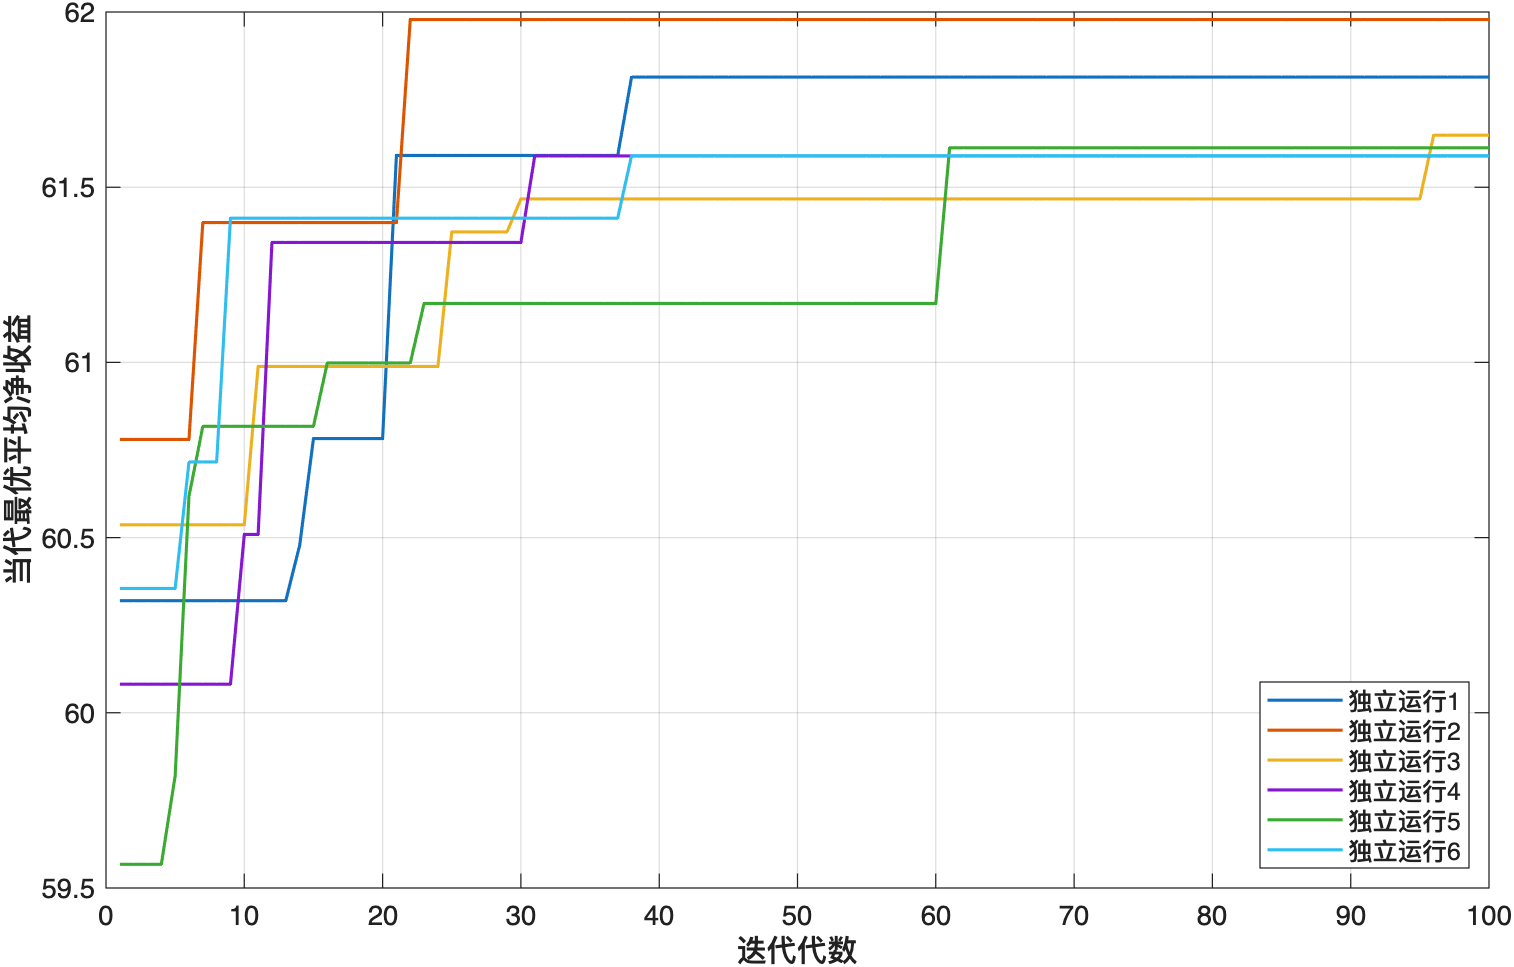
\includegraphics[width=0.86\linewidth]{../../第三问/results/ga_convergence.png}
  \caption{问题三6次独立遗传算法的最优适应度收敛曲线}
  \label{fig:p3-ga}
\end{figure}

至第100代时，6条曲线均进入稳定区间。6次搜索中有5次在修复后得到最终编码，命中率为83.33\%。另一次得到的边界策略在300000次复评下收益为60.0061元，低于最终策略的60.1574元。多次搜索与统一复评降低了单次GA随机性和1200次适应度样本波动对结果排序的影响。

\subsection{本问小结}

本文在问题二随机生产闭环的基础上，增加半成品质量、回收半成品及其内部零配件状态，建立两道工序下的分层随机生产闭环模型。通过蒙特卡洛评价、6次遗传算法搜索和300000次候选复评，得到策略 \texttt{11111111\textbar{}\allowbreak111\textbar{}\allowbreak0\textbar{}\allowbreak111\textbar{}\allowbreak1\textbar{}\allowbreak00000000\textbar{}\allowbreak11111111\textbar{}\allowbreak000\textbar{}\allowbreak111}，平均净收益为60.1574元/次合格交付。

该方案在采购端检测全部零配件，在工序间检测全部半成品，但不检测成品；两层不合格品均拆解，回收零配件和半成品利用已有质量信息直接回用。理论次数、规则基准和独立搜索结果均支持上述决策。该分层状态转移结构可继续用于问题四的策略求解。

\FloatBarrier

\section{问题四的建模与解决}

\subsection{问题分析}

\subsubsection{题目要求与数学本质}

问题四要求在零配件、半成品和成品次品率均由抽样检测获得的条件下，重新确定两类生产系统中的检测、拆解和回收策略。题给次品率不再是可直接代入的真实参数，而是有限样本形成的统计估计。抽样可能高估或低估实际质量风险，若仍把表中数值作为确定常数，所得策略只对单一参数点最优，无法回答抽样误差范围内应如何决策。

本问的输入包括题给样本次品率、各环节成本、售价、调换损失以及生产装配结构；需要输出各次品率的合理取值范围、该范围内的生产决策和对应收益。其数学本质是带有次品率取值范围的二进制决策问题：先由有限抽样推断真实次品率，再把参数区间传入随机生产闭环，最后从二进制策略空间中选择在次品率偏高时仍能保持较高收益的方案。

题目中的不确定性分为不同层次。真实次品率未知属于参数认知误差；给定次品率后，每件产品是否合格属于生产随机性；有限次仿真与真实期望之间的差异属于数值估计误差。三者不能由同一个概率量替代，因而需要分别建模：参数层给出置信范围，生产层模拟质量状态和成本累积，数值层用大样本复评控制误差。

\subsubsection{模型选择依据}

处理抽样次品率最直接的办法是将样本比例作为点估计代入收益模型。这种方法计算简单，但相同的样本比例可能由不同样本量得到，点估计不能反映其可信程度，也无法衡量参数偏差是否会改变最优策略。另一种选择是为次品率指定先验分布并建立贝叶斯随机规划，但题目没有提供历史先验或不同参数的联合分布，额外设定分布会引入无法由题目检验的参数。

区间方法只需要样本量和样本次品数，能够直接表达有限抽样造成的参数范围，更符合本题信息条件。由于样本量有限，且次品率包含5\%这类低概率取值，正态近似在分布尾部可能产生偏差，因此采用基于二项分布的Clopper--Pearson精确置信区间。生产系统包含多个次品率，分别构造95\%边际区间不足以保证所有参数同时被覆盖，故采用Bonferroni修正形成联合95\%置信域。

获得参数区间后，可以比较区间中心、上下界和内部情景，也可以直接优化各情景的平均收益。题目没有给出不同次品率情景的发生概率，若对情景赋予人为权重，结果会依赖权重设定。因此，本文用区间内可能出现的最低期望收益评价每个策略：先找出一个策略在参数区间内的最低收益，再从全部策略中选择最低收益最高的方案。该准则不需要人为设定情景概率，并能直接回答``当真实次品率高于表中估计值时，应采用何种生产策略''。

生产收益由采购、检测、装配、市场调换、拆解和回收循环共同决定，难以写成简单显式函数。本文使用随机生产闭环和蒙特卡洛模拟计算给定策略的期望收益。问题二有效策略数量较少，采用完全枚举获得最优决策；问题三包含38个二进制位，策略空间达到 \(2^{38}\)，采用遗传算法搜索并以独立大样本统一复评。计算过程依次完成次品率区间估计、最低情景收益计算、生产闭环模拟和策略搜索。

\subsubsection{建模路线}

根据上述分析，本问先把题给次品率视为样本估计，按抽样方案确定样本量并反推整数次品数；随后构造Bonferroni修正的精确二项区间，并以各参数区间的笛卡尔积表示联合取值范围。对任一生产策略，在给定参数情景下模拟从采购到合格交付的完整闭环，以长期平均净收益作为评价量；再以联合置信范围中的最低期望收益为目标，分别通过完全枚举和遗传算法确定两类生产系统的决策。最后使用中心、边界和区间内部情景复评，检查最低收益是否出现在联合上界，并估计蒙特卡洛误差。总体路线为

\[
\begin{aligned}
\text{样本次品率}
&\longrightarrow\text{样本量与次品数}
\longrightarrow\text{联合置信区间}\\
&\longrightarrow\text{最低情景收益目标}
\longrightarrow\text{生产策略优化与复评}.
\end{aligned}
\]

\subsubsection{质量参数口径与模型边界}

零配件次品率表示采购零配件本身不合格的概率。半成品和成品次品率均解释为合格投入条件下，当前装配工序自身产生次品的概率。设半成品 \(j\) 的零配件集合为 \(\mathcal G_j\)，其质量状态为

\[
G_j^{(s)}=
\left(\prod_{i\in\mathcal G_j}G_i^{(c)}\right)A_j^{(s)},
\qquad
P\left(A_j^{(s)}=0\right)=p_j^{(s)}.
\]

三个半成品装配为成品后，有

\[
G^{(f)}=
\left(\prod_{j=1}^{3}G_j^{(s)}\right)A^{(f)},
\qquad
P\left(A^{(f)}=0\right)=p_f.
\]

该定义将上游投入缺陷与当前工序失效分开，使每类抽样数据均对应唯一的模型参数。生产闭环假设不同质量事件相互独立，检测结果完全准确，拆解不改变组成对象质量，一份订单的销售收入只计一次，调换损失和替换品的重新生产成本均计入周期成本。

\subsection{抽样数据重构与联合置信区间}

\subsubsection{样本量与次品数}

题目未给出各类对象的实际样本量和样本次品数。按照问题一的抽样方案，本文将表中次品率 \(\hat p_j\) 视为样本估计，并分别计算接收与拒收方案的推荐样本量。为了形成一组用于参数估计的抽样记录，取二者中的较大者：

\[
n_j=\max\left\{n_j^{(a)},n_j^{(r)}\right\}.
\]

由于样本次品数必须为整数，按下式反推：

\[
x_j=\operatorname{round}(n_j\hat p_j).
\]

三种题给次品率对应的样本量和次品数见表8-1。10\%次品率对应 \(n=105,x=11\)，故实际用于区间计算的样本比例为 \(11/105\approx10.476\%\)；中心情景仍按题给10\%取值，该差异来自整数化处理。

\begin{longtable}[]{@{}
  >{\raggedleft\arraybackslash}p{(\linewidth - 8\tabcolsep) * \real{0.2000}}
  >{\raggedleft\arraybackslash}p{(\linewidth - 8\tabcolsep) * \real{0.2000}}
  >{\raggedleft\arraybackslash}p{(\linewidth - 8\tabcolsep) * \real{0.2000}}
  >{\raggedleft\arraybackslash}p{(\linewidth - 8\tabcolsep) * \real{0.2000}}
  >{\raggedleft\arraybackslash}p{(\linewidth - 8\tabcolsep) * \real{0.2000}}@{}}
\caption{题给次品率对应的抽样记录}\\
\toprule\noalign{}
\begin{minipage}[b]{\linewidth}\raggedleft
题给次品率
\end{minipage} & \begin{minipage}[b]{\linewidth}\raggedleft
拒收推荐样本量
\end{minipage} & \begin{minipage}[b]{\linewidth}\raggedleft
接收推荐样本量
\end{minipage} & \begin{minipage}[b]{\linewidth}\raggedleft
最终样本量 \(n\)
\end{minipage} & \begin{minipage}[b]{\linewidth}\raggedleft
次品数 \(x\)
\end{minipage} \\
\midrule\noalign{}
\endfirsthead
\toprule\noalign{}
\begin{minipage}[b]{\linewidth}\raggedleft
题给次品率
\end{minipage} & \begin{minipage}[b]{\linewidth}\raggedleft
拒收推荐样本量
\end{minipage} & \begin{minipage}[b]{\linewidth}\raggedleft
接收推荐样本量
\end{minipage} & \begin{minipage}[b]{\linewidth}\raggedleft
最终样本量 \(n\)
\end{minipage} & \begin{minipage}[b]{\linewidth}\raggedleft
次品数 \(x\)
\end{minipage} \\
\midrule\noalign{}
\endhead
\bottomrule\noalign{}
\endlastfoot
5\% & 94 & 106 & 106 & 5 \\
10\% & 85 & 105 & 105 & 11 \\
20\% & 77 & 79 & 79 & 16 \\
\end{longtable}

表8-1中的样本量由问题一的临界比例标准差稳定性规则确定，因此其大小不能解释为一般意义上的估计精度排序。

\subsubsection{精确二项置信区间}

设第 \(j\) 类对象抽取 \(n_j\) 件，其中有 \(X_j\) 件次品，则

\[
X_j\sim\operatorname{Bin}(n_j,p_j),
\]

其中 \(p_j\) 为未知总体次品率。观察到 \(X_j=x_j\) 后，采用 Clopper--Pearson 精确二项区间。给定单参数显著性水平 \(\alpha_j\)，区间下限和上限分别为

\[
p_j^L=B^{-1}\left(\frac{\alpha_j}{2};x_j,n_j-x_j+1\right),
\]

\[
p_j^U=B^{-1}\left(1-\frac{\alpha_j}{2};x_j+1,n_j-x_j\right),
\]

其中 \(B^{-1}(q;a,b)\) 表示参数为 \((a,b)\) 的Beta分布在概率 \(q\) 处的分位数。该区间直接依据二项分布计算，不使用正态近似，适用于本题有限样本和低次品率情形。

\subsubsection{Bonferroni联合修正}

问题二和问题三需要同时估计多个次品率。若各参数分别使用95\%区间，所有真实参数同时落入对应区间的概率不能保证达到95\%。设同一优化问题包含 \(d\) 个次品率参数，总体显著性水平为 \(\alpha=0.05\)，本文令

\[
\alpha_j=\frac{0.05}{d},\qquad j=1,2,\ldots,d.
\]

由Bonferroni不等式可得

\[
P\left(p_1\in I_1,\ldots,p_d\in I_d\right)
\geq 1-\sum_{j=1}^{d}\alpha_j=0.95.
\]

问题二的每种情形含两个零配件次品率和一个成品工序次品率，故 \(d=3\)；六种情形是六个独立的生产环境，分别进行三参数联合修正。问题三包含8个零配件次品率、3个半成品工序次品率和1个成品工序次品率，故 \(d=12\)。相应区间见表8-2。

\begin{longtable}[]{@{}lrrc@{}}
\caption{Bonferroni修正后的次品率区间}\\
\toprule\noalign{}
使用位置 & 参数个数 \(d\) & 题给次品率 & 精确置信区间 \\
\midrule\noalign{}
\endfirsthead
\toprule\noalign{}
使用位置 & 参数个数 \(d\) & 题给次品率 & 精确置信区间 \\
\midrule\noalign{}
\endhead
\bottomrule\noalign{}
\endlastfoot
问题二 & 3 & 5\% & {[}0.011683, 0.121363{]} \\
问题二 & 3 & 10\% & {[}0.045429, 0.197320{]} \\
问题二 & 3 & 20\% & {[}0.106305, 0.331524{]} \\
问题三 & 12 & 10\% & {[}0.037684, 0.217293{]} \\
\end{longtable}

问题三对12个参数同时提供覆盖保证，单参数显著性水平降为 \(0.05/12\)，故其10\%次品率区间比问题二的三参数区间更宽。

\subsubsection{抽样成本口径}

问题一和问题四中的抽样检测用于识别一批产品的质量参数，问题二、三中的生产检测则用于判断某个具体零配件、半成品或成品能否进入下一工序。两类检测的作用对象不同。若批次规模为 \(M\)、抽样总成本为 \(C_{\mathrm{sample}}\)，其单位分摊成本应为 \(C_{\mathrm{sample}}/M\)。题目未给出批次规模及单独的抽样费用，无法将该项成本换算到一次合格交付，因此本文不把抽样成本重复计入问题二、三的周期收益；表中检测成本仍按原生产决策模型逐件核算。

\subsection{联合置信上界下的决策模型}

\subsubsection{次品率的联合取值范围}

设同一生产问题的次品率向量为

\[
\boldsymbol p=(p_1,p_2,\ldots,p_d),
\]

由各参数精确置信区间构造联合取值范围

\[
\Theta=\prod_{j=1}^{d}[p_j^L,p_j^U]
=\left\{\boldsymbol p:p_j^L\leq p_j\leq p_j^U,\ j=1,\ldots,d\right\}.
\]

对生产策略 \(S\)，沿用前文的周期净收益

\[
R(S)=V-C_{\mathrm{purchase}}-C_{\mathrm{inspection}}
-C_{\mathrm{assembly}}-C_{\mathrm{return}}-C_{\mathrm{disassembly}}.
\]

在给定次品率向量 \(\boldsymbol p\) 时，其期望收益为

\[
F(S;\boldsymbol p)=E[R(S)\mid S,\boldsymbol p].
\]

记按表中次品率选择的策略为 \(S_{\hat p}^*\)，按联合置信范围内最低收益选择的策略为 \(S_U^*\)，分别定义为

\[
S_{\hat p}^*
=\arg\max_{S\in\Omega}F(S;\hat{\boldsymbol p}),
\]

\[
S_U^*
=\arg\max_{S\in\Omega}
\min_{\boldsymbol p\in\Theta}F(S;\boldsymbol p).
\]

第一个策略只考虑题目表中给出的次品率。第二个策略的含义是：对每个候选策略，先计算其在联合置信范围内可能得到的最低收益，再比较所有候选策略的这一最低收益，并选择数值最大者。下文将二者分别简称为``表中次品率策略''和``上界情景策略''。这里的``上界情景策略''不是另一套生产模型，而是把真实次品率同时取到各自置信区间的上界后，仍用同一个生产闭环收益模型选择策略。

\subsubsection{最低收益情景的确定}

在既定生产策略下，提高某个次品率会使部分原本合格的质量状态转为不合格，并增加重复采购、检测淘汰、重复装配、市场调换或拆解循环。销售收入对一份订单只计一次，缺陷本身不产生额外收益，回收只能抵消部分新增成本。因此，在本文假设下，固定策略的期望收益关于各次品率均为非增函数，即

\[
p_j^{(1)}\leq p_j^{(2)}
\quad\Longrightarrow\quad
F(S;p_j^{(1)})\geq F(S;p_j^{(2)}).
\]

于是，联合置信范围内的最低收益出现在全部参数同时取上界时：

\[
\boldsymbol p^U=(p_1^U,p_2^U,\ldots,p_d^U),
\]

\[
\min_{\boldsymbol p\in\Theta}F(S;\boldsymbol p)
=F(S;\boldsymbol p^U).
\]

因此，前述``先求区间内最低收益、再比较策略''的计算可化为

\[
S_U^*
=\arg\max_{S\in\Omega}F(S;\boldsymbol p^U).
\]

这一步只是利用收益随次品率上升而不增加的性质，将区间内搜索简化为联合上界处的一次评价，并未改变原来的选择准则。中心、联合下界、单参数上下界和区间内部拉丁超立方情景仅用于检验该单调性及比较策略表现，不参与策略目标的重新定义。

\subsubsection{两类策略的收益差额}

为衡量改用上界情景策略后在表中次品率情景下的收益变化，定义中心情景收益差

\[
\Delta F_{\mathrm{center}}=
F(S_{\hat p}^*;\hat{\boldsymbol p})
-F(S_U^*;\hat{\boldsymbol p}).
\]

该量表示从表中次品率策略转为上界情景策略后，在表中次品率下减少的平均收益。进一步定义联合上界收益增量

\[
\Delta F_{\mathrm{upper}}=
F(S_U^*;\boldsymbol p^U)
-F(S_{\hat p}^*;\boldsymbol p^U),
\]

用于衡量改用上界情景策略后，在所有次品率同时取置信上界时增加的平均收益。

\subsection{问题二在次品率区间下的决策优化}

\subsubsection{求解方法}

问题二的生产策略采用8位编码

\[
x_1x_2\mid yz\mid r_1r_2\mid u_1u_2.
\]

经无效决策修复后共有80种有效策略。对表1的六种情形，本文分别计算三参数联合区间，将对应上界代入原随机生产闭环，并对80种策略各进行100000次蒙特卡洛仿真，以联合上界情景下的平均净收益确定上界情景策略。随后在中心、联合上下界、6个单参数边界及64个拉丁超立方内部情景中进行复评，每个验证情景使用30000次仿真。

\subsubsection{两类策略的计算结果}

六种情形在表中次品率和联合上界下选出的策略见表8-3。表中同时列出上界情景策略在联合上界下的收益、中心情景收益差和联合上界收益增量。

\begin{longtable}[]{@{}
  >{\raggedleft\arraybackslash}p{(\linewidth - 10\tabcolsep) * \real{0.1538}}
  >{\centering\arraybackslash}p{(\linewidth - 10\tabcolsep) * \real{0.1923}}
  >{\centering\arraybackslash}p{(\linewidth - 10\tabcolsep) * \real{0.1923}}
  >{\raggedleft\arraybackslash}p{(\linewidth - 10\tabcolsep) * \real{0.1538}}
  >{\raggedleft\arraybackslash}p{(\linewidth - 10\tabcolsep) * \real{0.1538}}
  >{\raggedleft\arraybackslash}p{(\linewidth - 10\tabcolsep) * \real{0.1538}}@{}}
\caption{问题二表中次品率策略与上界情景策略比较}\\
\toprule\noalign{}
\begin{minipage}[b]{\linewidth}\raggedleft
情形
\end{minipage} & \begin{minipage}[b]{\linewidth}\centering
表中次品率策略
\end{minipage} & \begin{minipage}[b]{\linewidth}\centering
上界情景策略
\end{minipage} & \begin{minipage}[b]{\linewidth}\raggedleft
上界策略收益/元
\end{minipage} & \begin{minipage}[b]{\linewidth}\raggedleft
中心情景收益差/元
\end{minipage} & \begin{minipage}[b]{\linewidth}\raggedleft
联合上界收益增量/元
\end{minipage} \\
\midrule\noalign{}
\endfirsthead
\toprule\noalign{}
\begin{minipage}[b]{\linewidth}\raggedleft
情形
\end{minipage} & \begin{minipage}[b]{\linewidth}\centering
表中次品率策略
\end{minipage} & \begin{minipage}[b]{\linewidth}\centering
上界情景策略
\end{minipage} & \begin{minipage}[b]{\linewidth}\raggedleft
上界策略收益/元
\end{minipage} & \begin{minipage}[b]{\linewidth}\raggedleft
中心情景收益差/元
\end{minipage} & \begin{minipage}[b]{\linewidth}\raggedleft
联合上界收益增量/元
\end{minipage} \\
\midrule\noalign{}
\endhead
\bottomrule\noalign{}
\endlastfoot
1 & \texttt{10\textbar{}\allowbreak01\textbar{}\allowbreak01\textbar{}\allowbreak11} & \texttt{11\textbar{}\allowbreak01\textbar{}\allowbreak00\textbar{}\allowbreak11} & 12.1314 & 0.7247 & 1.8740 \\
2 & \texttt{11\textbar{}\allowbreak01\textbar{}\allowbreak00\textbar{}\allowbreak11} & \texttt{11\textbar{}\allowbreak01\textbar{}\allowbreak00\textbar{}\allowbreak11} & 1.2041 & 0 & 0 \\
3 & \texttt{10\textbar{}\allowbreak11\textbar{}\allowbreak01\textbar{}\allowbreak11} & \texttt{11\textbar{}\allowbreak11\textbar{}\allowbreak00\textbar{}\allowbreak11} & 9.8932 & 1.0648 & 1.1272 \\
4 & \texttt{11\textbar{}\allowbreak11\textbar{}\allowbreak00\textbar{}\allowbreak11} & \texttt{11\textbar{}\allowbreak11\textbar{}\allowbreak00\textbar{}\allowbreak11} & 5.6496 & 0 & 0 \\
5 & \texttt{01\textbar{}\allowbreak01\textbar{}\allowbreak00\textbar{}\allowbreak01} & \texttt{01\textbar{}\allowbreak11\textbar{}\allowbreak00\textbar{}\allowbreak01} & 6.1800 & 0.0316 & 2.4341 \\
6 & \texttt{00\textbar{}\allowbreak00\textbar{}\allowbreak00\textbar{}\allowbreak00} & \texttt{10\textbar{}\allowbreak00\textbar{}\allowbreak00\textbar{}\allowbreak00} & 13.1547 & 0.3474 & 3.2313 \\
\end{longtable}

\begin{figure}[htbp]
  \centering
  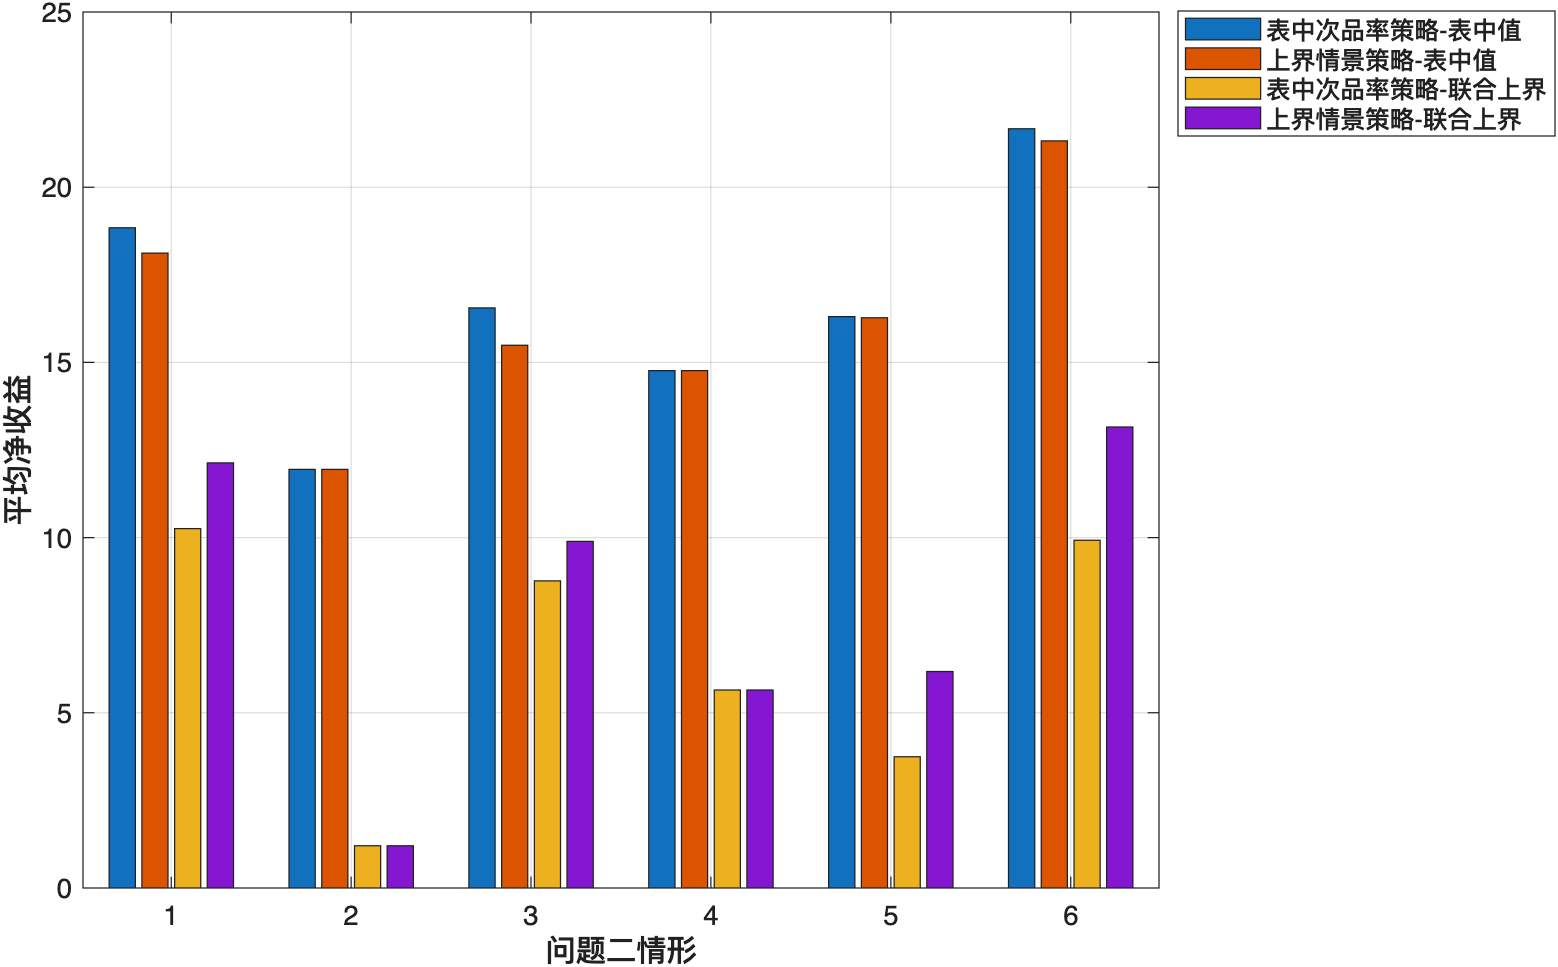
\includegraphics[width=0.86\linewidth]{../../第四问/results_problem2/profit_comparison.png}
  \caption{问题二两类策略在表中次品率及联合上界情景下的收益比较}
  \label{fig:p4-p2-profit}
\end{figure}

\subsubsection{决策变化分析}

情形1和情形3的上界情景策略均增加了新购零配件2检测。10\%样本估计对应的联合上界为19.732\%，不检测零配件2时，坏件进入装配并引发重复生产的概率上升。将检测前移至采购端后，零配件2以确定合格状态进入装配；在检测准确、拆解无损的条件下，回收后也无需重复检测。因此编码由回收检测位 \(01\) 转为新件检测位 \(11\)、回收检测位 \(00\)。

情形2和情形4的策略未发生变化。两种原策略均已检测两个新购零配件；情形4还检测成品，原决策已覆盖联合上界下主要的质量风险。情形2的成品调换损失较低，持续支付成品检测费不能提高联合上界下的期望收益，故仍不检测成品。

情形5只增加成品检测。上界情景策略仍检测零配件2而不检测零配件1，但零配件1和成品工序的次品率均可能达到19.732\%。在零配件2已知合格时，零配件1缺陷与成品工序失效叠加后的成品次品概率约为

\[
1-(1-0.197320)^2\approx0.3556,
\]

高于表中次品率下的 \(1-(1-0.1)^2=0.19\)。此时支付2元进行成品检测比承担10元市场调换损失更有利。该调整使表中次品率下的平均收益减少0.0316元，同时使联合上界下的平均收益增加2.4341元。

情形6的题给次品率为5\%，表中次品率策略不进行任何检测、拆解和回收。联合上界提高至12.136\%后，完全不检测的重复生产风险增大，上界情景策略增加检测成本较低的零配件1，但零配件2检测、成品检测和高成本拆解仍不经济。该调整使表中次品率下的平均收益减少0.3474元，但使联合上界下的平均收益增加3.2313元，是六种情形中收益变化最明显的一种。

\subsection{问题三在次品率区间下的决策优化}

\subsubsection{参数情景与遗传算法}

问题三的12个次品率样本估计均为10\%，经联合修正后有

\[
p_j\in[0.037684,0.217293],\qquad j=1,2,\ldots,12.
\]

问题三的生产策略采用38位二进制编码，并根据拆解、利用及已知质量状态清除无效决策位。在全部次品率取上界0.217293的情景下运行遗传算法。搜索采用种群80、100代、交叉概率0.8、变异概率0.03、锦标赛规模3和精英数2；每次适应度使用1200个生产周期，共独立运行6次，每次保留10个候选。合并去重后，对候选策略进行300000次独立仿真复评。

\subsubsection{策略与收益比较}

按表中次品率选择的策略为

\[
11111111\mid111\mid0\mid111\mid1
\mid00000000\mid11111111\mid000\mid111,
\]

按联合上界选择的策略为

\[
11111111\mid111\mid1\mid111\mid1
\mid00000000\mid11111111\mid000\mid111.
\]

两者仅在成品检测位上不同。上界情景策略检测全部新购零配件、三个半成品及成品；三类不合格半成品和不合格成品均拆解；回收零配件与回收半成品不重复检测，全部重新利用。核心收益见表8-4。

\begin{longtable}[]{@{}
  >{\raggedright\arraybackslash}p{(\linewidth - 6\tabcolsep) * \real{0.2353}}
  >{\raggedleft\arraybackslash}p{(\linewidth - 6\tabcolsep) * \real{0.2353}}
  >{\raggedleft\arraybackslash}p{(\linewidth - 6\tabcolsep) * \real{0.2353}}
  >{\centering\arraybackslash}p{(\linewidth - 6\tabcolsep) * \real{0.2941}}@{}}
\caption{问题三表中次品率策略与上界情景策略的收益比较}\\
\toprule\noalign{}
\begin{minipage}[b]{\linewidth}\raggedright
策略
\end{minipage} & \begin{minipage}[b]{\linewidth}\raggedleft
中心情景收益/元
\end{minipage} & \begin{minipage}[b]{\linewidth}\raggedleft
联合上界收益/元
\end{minipage} & \begin{minipage}[b]{\linewidth}\centering
联合上界95\%蒙特卡洛区间/元
\end{minipage} \\
\midrule\noalign{}
\endfirsthead
\toprule\noalign{}
\begin{minipage}[b]{\linewidth}\raggedright
策略
\end{minipage} & \begin{minipage}[b]{\linewidth}\raggedleft
中心情景收益/元
\end{minipage} & \begin{minipage}[b]{\linewidth}\raggedleft
联合上界收益/元
\end{minipage} & \begin{minipage}[b]{\linewidth}\centering
联合上界95\%蒙特卡洛区间/元
\end{minipage} \\
\midrule\noalign{}
\endhead
\bottomrule\noalign{}
\endlastfoot
表中次品率策略 & 60.1753 & 29.1258 & --- \\
上界情景策略 & 58.0771 & 32.6135 & {[}32.5093, 32.7177{]} \\
\end{longtable}

上界情景策略相对于表中次品率策略的中心情景收益差为

\[
\Delta F_{\mathrm{center}}=60.1753-58.0771=2.0982\text{元},
\]

联合上界收益增量为

\[
\Delta F_{\mathrm{upper}}=32.6135-29.1258=3.4877\text{元}.
\]

因此，增加成品检测使表中次品率下的平均收益下降2.0982元，但使所有次品率同时取置信上界时的平均收益提高3.4877元。

\subsubsection{成品检测决策的转换机理}

表中次品率策略已经检测全部新购零配件和半成品，故进入最终装配的半成品均为合格状态，剩余质量风险集中在成品装配工序。设其失效率为 \(p_f\)。若检测成品，每完成一件合格交付所需的理论检测费用为

\[
C_{\mathrm{inspect}}=\frac{6}{1-p_f}.
\]

若不检测成品，每次不合格均进入市场，完成一件合格交付前的理论调换损失为

\[
C_{\mathrm{return}}=40\frac{p_f}{1-p_f}.
\]

两者的临界条件为

\[
\frac{6}{1-p_f}<40\frac{p_f}{1-p_f}
\quad\Longleftrightarrow\quad
p_f>0.15.
\]

表中数值 \(p_f=0.10\) 低于临界值，因此对应策略不检测成品；联合上界 \(p_f^U=0.217293\) 高于临界值，上界情景策略转为检测成品。以两种参数代入，可得

\[
p_f=0.10:\quad
C_{\mathrm{inspect}}=6.6667,
\quad C_{\mathrm{return}}=4.4444,
\]

\[
p_f=0.217293:\quad
C_{\mathrm{inspect}}\approx7.666,
\quad C_{\mathrm{return}}\approx11.105.
\]

该理论比较与遗传算法给出的检测位变化一致。回收对象仍不重复检测，是因为新购零配件和半成品已通过检测，且无损拆解不改变质量；再次检测只增加成本，不增加质量信息。

\subsection{结果检验}

\subsubsection{情景边界检验}

问题二对每种情形构造中心、联合上下界、6个单参数边界和64个拉丁超立方内部情景；问题三构造中心、联合上下界、24个单参数边界和128个拉丁超立方内部情景。对表中次品率策略和上界情景策略分别进行独立复评后，所有问题二情形以及问题三的最低平均收益均出现在联合上界情景，与收益关于次品率非增的机理判断一致。

\subsubsection{蒙特卡洛精度与重复搜索结果}

问题二对全部80种有效策略进行100000次仿真，故最终结果来自全枚举而非启发式近似。问题三无法枚举 \(2^{38}\) 个原始编码，采用6次独立遗传搜索。图8-2给出了联合上界情景下的收敛过程。

\begin{figure}[htbp]
  \centering
  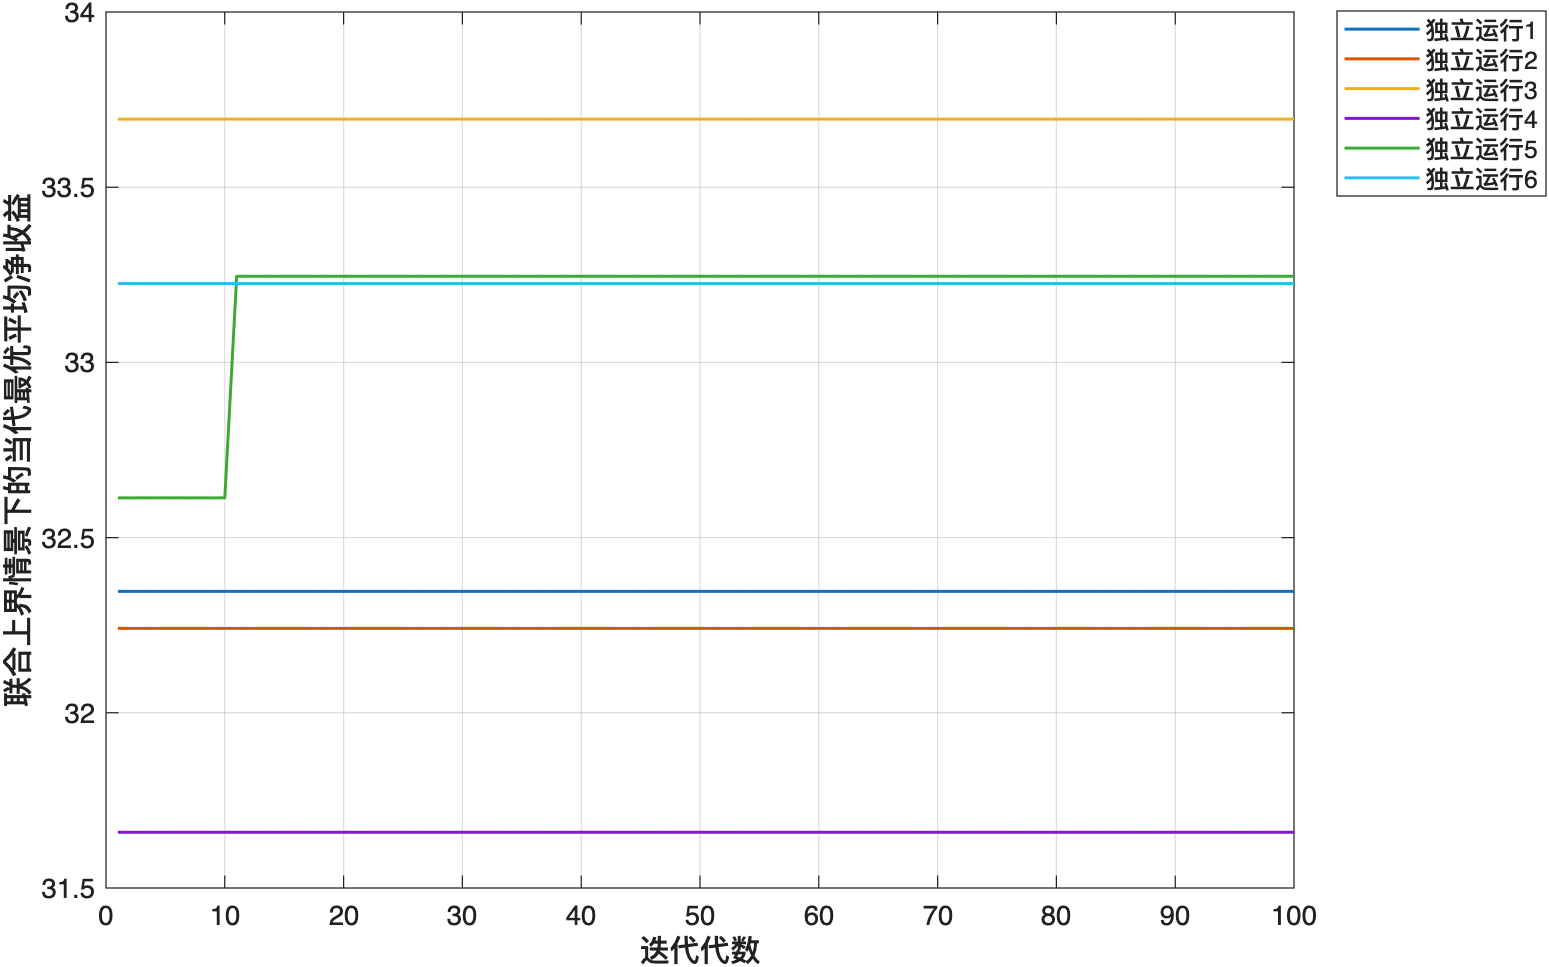
\includegraphics[width=0.86\linewidth]{../../第四问/results_problem3/ga_convergence.png}
  \caption{问题三联合上界情景下6次遗传算法收敛曲线}
  \label{fig:p4-p3-ga}
\end{figure}

6次搜索中有5次得到最终采用的上界情景编码，第5次得到的另一候选策略仅将回收零配件1由利用改为废弃。300000次统一复评下，最终策略的联合上界收益为32.6135元，另一候选策略为31.4421元，表中次品率策略约为29.04元。最终策略的95\%蒙特卡洛区间宽度约为0.2084元，且全部正式验证样本的闭环完成率均为1，说明循环上限没有影响入选策略的收益评价。

由于问题三使用启发式搜索，最终方案应表述为``在6次独立搜索中重复出现，并在大样本统一复评中收益最高的候选策略''，不作严格全局最优声明。

\subsection{本问小结}

本文先把题给次品率视为样本估计，根据既定选样规则反推样本次品数，再使用Bonferroni修正的Clopper--Pearson精确区间构造联合95\%次品率取值范围。由于固定策略的收益随次品率上升而不增加，区间内的最低收益出现在所有次品率同时取上界时，因而在联合上界情景下选择检测、拆解和回收策略。

问题二的六种情形中，情形2和4的两类策略相同，情形1和3的上界情景策略增加新购零配件2检测，情形5增加成品检测，情形6增加新购零配件1检测。问题三的上界情景策略在表中次品率策略的基础上增加成品检测，表中次品率下的收益由60.1753元降至58.0771元，但联合上界收益由29.1258元提高至32.6135元。结果表明，抽样误差不会使所有环节一律转为检测，而会使决策在容易放大质量损失的环节增加检测。

\FloatBarrier

% 后续待补：模型评价与推广、参考文献、附录。
\end{document}
